\documentclass[
%dbse, % include logo of DBSE work group
    %draft,    % omit title page, listings, and particular chapters selected below using include only
	german,   % titles for a thesis in German, A4 paper
	%print,    % the printed version does not use colored links
	%final,    % removes all TODOs
]{tex/ttthesis}

% Color Scheme http://colorschemedesigner.com/#3w40I--ALK-K-
% Base Color of the OVGU INF logo, tetraed, -45
\definecolor{blue1}{RGB}{0,105,180} % gray 95
\definecolor{blue2}{RGB}{40,87,121}
\definecolor{blue3}{RGB}{0,57,97}
\definecolor{blue4}{RGB}{76,166,230}
\definecolor{blue5}{RGB}{136,191,230}
\definecolor{orange1}{RGB}{255,144,0} % gray 133
\definecolor{orange2}{RGB}{171,121,56}
\definecolor{orange3}{RGB}{137,78,0}
\definecolor{orange4}{RGB}{255,181,84}
\definecolor{orange5}{RGB}{255,210,151}
\definecolor{green1}{RGB}{11,215,0} % gray 75
\definecolor{green2}{RGB}{52,144,48}
\definecolor{green3}{RGB}{6,116,0}
\definecolor{green4}{RGB}{88,241,80}
\definecolor{green5}{RGB}{148,241,143}
\definecolor{red1}{RGB}{253,0,6} % gray 86
\definecolor{red2}{RGB}{170,56,59}
\definecolor{red3}{RGB}{136,0,3}
\definecolor{red4}{RGB}{254,84,88}
\definecolor{red5}{RGB}{254,151,154}

\definecolor{background}{named}{white}
\definecolor{bgborder}{named}{black}
\definecolor{comment}{named}{red3}

\definecolor{blue}{named}{blue1}
\definecolor{green}{named}{green1}
\definecolor{red}{named}{red1}
\definecolor{orange}{named}{orange1}

\definecolor{pdflinkcolor}{named}{blue3}
\definecolor{pdfcitecolor}{named}{green3}

\usepackage{listings} % source code listings

%\renewcommand\lstlistingname{Quelltext}

\lstdefinestyle{java}{
%code formatting
	language=Java,
	tabsize=4,
	breaklines=false,
	basicstyle=\fontfamily{pcr}\footnotesize\selectfont,
	commentstyle=\fontshape{it}\color{darkgray}\selectfont,
	keywordstyle=\fontseries{b}\selectfont,
	stringstyle=\fontfamily{cmr}\selectfont,
%line numbering
	numbers=left,
	numberstyle=\footnotesize,
%frame properties
	captionpos=b,
	frame=single,%trblTRBL
	framesep=3pt,
	xleftmargin=4pt,
	xrightmargin=4pt,
	rulecolor=\color{bgborder},
}

\usepackage{pgfplots}
\usepackage{tikz}
	\usetikzlibrary{arrows,positioning,backgrounds,fit,trees} 
	\usetikzlibrary{fadings,shapes.geometric}
	\usetikzlibrary{decorations,scopes,calc,decorations.pathreplacing}

% Tortendiagramme
\newcommand{\slice}[4]{
  \pgfmathparse{0.5*#1+0.5*#2}
  \let\midangle\pgfmathresult

  % slice
  \draw[thick,
	%fill=background
	] (0,0) -- (#1:1) arc (#1:#2:1) -- cycle;

  % outer label
  \node[label=\midangle:#4] at (\midangle:1) {};

  % inner label
  \pgfmathparse{min((#2-#1-10)/110*(-0.3),0)}
  \let\temp\pgfmathresult
  \pgfmathparse{max(\temp,-0.5) + 0.8}
  \let\innerpos\pgfmathresult
  \node at (\midangle:\innerpos) {#3};
}
\newcommand{\mypiechart}[2]{
	\begin{tikzpicture}[scale=#1]
		\newcounter{a}
		\newcounter{b}
		\foreach \p/\t in {#2}
			{
				\setcounter{a}{\value{b}}
				\addtocounter{b}{\p}
				\slice{\thea/100*360}
							{\theb/100*360}
							{\p\%}{\t}
			}
	\end{tikzpicture}
}

% surrounding TODOs with this command, gives you the ability to remove all if necessary
\iffinal{
	\newcommand{\todo}[1]{}
	\newcommand{\todots}{}
}{
	\newcommand{\todo}[1]{{\color{comment}\textit{[#1]}}}
	\newcommand{\todots}{\todo{\ldots}}
}

% propositional formulas
\newcommand{\pand}{\wedge}
\newcommand{\por}{\vee}
\newcommand{\pnot}{\neg}
\newcommand{\pequals}{\Leftrightarrow}
\newcommand{\pimplies}{\Rightarrow}
\newcommand{\pnimplies}{\nRightarrow}
\newcommand{\patmostone}{\mbox{\textit{atmost1}}}
\newcommand{\pchooseone}{\mbox{\textit{choose1}}}

% mathematical definitions and theorems
\newtheorem{definition}{Definition}[chapter]
\newtheorem{theorem}{Theorem}[chapter]
\newtheorem{lemma}{Lemma}[chapter]

% print URLs not in Typewriter Font
\def\UrlFont{\rm}

% empty page without page number, continue on the next right page
\newcommand{\blankpage}{\clearpage{\pagestyle{empty}\cleardoublepage}}

% index stuff
\makeatletter
\def\mydotfill{\leavevmode\xleaders\hb@xt@ .44em{\hss.\hss}\hfill\kern\z@}
\makeatother
\def\bold#1{{\bfseries #1}}
\newbox\dbox \setbox\dbox=\hbox to .4em{\hss.\hss} % dot box for leaders
\newskip\rrskipb \rrskipb=.5em plus3em % ragged right space before break
\newskip\rrskipa \rrskipa=-.17em plus -3em minus.11em % ditto, after
\newskip\rlskipa \rlskipa=0pt plus3em % ragged left space after break
\newskip\rlskipb \rlskipb=.33em plus-3em minus.11em % ragged left before break
\newskip\lskip \lskip=3.3\wd\dbox plus1fil minus.3\wd\dbox % for leaders
\newskip \lskipa \lskipa=-2.67em plus -3em minus.11em %after leaders
\mathchardef\rlpen=1000 \mathchardef\leadpen=600
\def\rrspace{\nobreak\hskip\rrskipb\penalty0\hskip\rrskipa}
\def\rlspace{\penalty\rlpen\hskip\rlskipb\vadjust{}\nobreak\hskip\rlskipa}
\let\indexbreak\rlspace
\def\raggedurl{\penalty10000 \hskip.5em plus15em \penalty0 \hskip-.17em plus-15em minus.11em}
\def\raggeditems{\nobreak\hskip\rrskipb \penalty\leadpen \hskip\rrskipa %
\vadjust{}\nobreak\leaders\copy\dbox\hskip\lskip %
\kern3em \penalty\leadpen \hskip\lskipa %
\vadjust{}\nobreak\hskip\rlskipa}
\renewcommand*\see[2]{\rlspace\emph{\seename}~#1} % from makeidx.sty


\usepackage{pdfpages}

%*********************************************************************%
% META                                                                %
%*********************************************************************%
\ifgerman{
  \newcommand{\university}{Otto-von-Guericke-Universität Magdeburg}
  \newcommand{\school}{Fakultät für Informatik}
}{
  \newcommand{\university}{University of Magdeburg}
  \newcommand{\school}{School of Computer Science}
}
\newcommand{\logo}{} %\includegraphics[trim=0mm 0mm 50mm 0mm,clip,height=3cm]{INF_SIGN_druck}}
\newcommand{\logodbse}{} %\includegraphics[scale=.45]{DBSE}}

\newcommand{\advisorone}{Jun.-Prof. Thorsten Grosch}
\newcommand{\departmentone}{\ifgerman{Institut für Simulation und Graphik}{Department of}}

\newcommand{\advisortwo}{Maria Manneck, Enrico Gebert}
\newcommand{\departmenttwo}{Acagamics e.V.}

% Thesis kind
\newcommand{\thesiskind}{Wissenschaftliche Ausarbeitung im Rahmen der Lehrveranstaltung Advanced Game Development 2013/14}
%\ifgerman{\newcommand{\thesiskind}{Bachelorarbeit}}{\newcommand{\thesiskind}{Bachelor Thesis}}
%\newcommand{\thesiskind}{Diplomarbeit} %do not translate
%\ifgerman{\newcommand{\thesiskind}{Doktorarbeit}}{\newcommand{\thesiskind}{Dissertation}}

\ifgerman{
	\newcommand{\authornames}{Johannes Jendersie, Florian Uhde, David Kuri}
	\newcommand{\thetitle}{\todo{Scarlet Gamma}}
	\newcommand{\thedate}{\todo{13. Monat}}
}{
	\newcommand{\authornames}{\todots}
	\newcommand{\thetitle}{\todo{The Title of the Thesis}}
	\newcommand{\thedate}{\todo{Month 13}}
}
\newcommand{\theyear}{2014}

%*********************************************************************%
% SETUP                                                               %
%*********************************************************************%

% meta informations of the document
\hypersetup{
 pdfauthor={\authornames},
 pdftitle={\thetitle}
}

% open index file
\ifnotdraft{\makeindex}

%*********************************************************************%
% ACRONYMS                                                            %
%*********************************************************************%

% HOWTO: \gls{IDE} for singular or \glspl{IDE} for plural with 's
\makeglossaries
\newacronym{RPG}{RPG}{Role Playing Game}
\glsaddall % use only if you have acronyms that occur only in graphics

%*********************************************************************%
% THE DOCUMENT                                                        %
%*********************************************************************%

\begin{document}

% set the path where graphics are located
\graphicspath{{pics/}}

\ifnotdraft{
	\frontmatter
	\pagenumbering{roman}
	\newcommand{\theauthor}{\theforename\ \thesurname}
\newcommand{\theauthorr}{\thesurname,\ \theforename}
\begin{titlepage}
 \thispagestyle{empty}
 \begin{center}
  {\university}\\[0.4cm]
  {\school}\\[2.0cm]
  \begin{figure}[h]
   \hbox{}\hfill
    \begin{minipage}[t]{\textwidth}
      \begin{center}
        \logo\ifdbse{\\[0.4cm]
        \logodbse
        }{ }
      \end{center}
    \end{minipage} 
   \hfill\hbox{}
  \end{figure}\ \\[0.4cm]
  \ifdbse{
  {\large \thesiskind \\[1cm]}
  {\huge\bf \thetitle \\[1cm]}
  }
  {
  {\large \thesiskind \\[1.6cm]}
  {\huge\bf \thetitle \\[1.6cm]}
  }
  { \ifgerman{Autor:}{Author:}}\\[0.4cm]
  {\huge \theauthor}\\[0.8cm]
  {\large\thedate, \theyear}\\[0.8cm]
  {\ifgerman{Betreuer:}{Advisors:}}\\[0.4cm] 
  {\large
\advisorone
  }\\[0.2cm]
  {
\departmentone
  }\\[0.8cm]
  {\large
\advisortwo\ 
  }\\[0.2cm]
  {
\departmenttwo\ 
  }
 \end{center}
\end{titlepage}

%%%%%%%%%%%%%%%%%%%%%%%%%%%%%%%%%%%%%%%%%%%%%%%%%%%%%%%%%%%%%%%%%%%%%%%%%%%%
%%% Titelrückseite: Bibliographische Angaben
%%%%%%%%%%%%%%%%%%%%%%%%%%%%%%%%%%%%%%%%%%%%%%%%%%%%%%%%%%%%%%%%%%%%%%%%%%%%

\thispagestyle{empty}
\vspace*{\fill}
\begin{minipage}{15.0cm}
\textbf{\theauthorr:}\\
\emph{\thetitle\\}
\thesiskind, \university, \theyear.
\end{minipage}
%\newpage

	% TODO: Put on the backside of title page
	%\chapter*{Inhaltsangabe}

Bei vielen modernen PC-Rollenspielen tritt die Schwierigkeit auf dem Spieler Handlungsfreiraum einzuräumen. Es stellt sich die Frage, ob es nicht möglich ist die Freiheit, die es im Vorgänger, den Pen-\&-Paper-Spielen, gab zu übertragen. Es gibt unterschiedlich Ansätze in die Richtung die Handlung dynamisch anzupassen.

Wir beschäftigen uns hingegen mit der Frage, ob der Computer überhaupt als Medium in Frage kommt. Dazu übertragen wir das Pen-\&-Paper-Spiel direkt und fordern, dass einer der Spieler die Sonderrolle des allmächtigen Spielleiters übernimmt. Der von uns entwickelte Prototyp versucht weitestgehend viel Komfort zu bieten und gleichzeitig die Spieler nicht in ihrem Handlungsfreiraum einzuschränken. Wir haben dazu eine Komponenten basierte Welt in ein Multiplayer-Spiel eingebettet und in Nutzertests evaluiert. Das Ziel der Handlungsfreiheit wurde erreicht und es hat sich gezeigt, dass der Computer gleichzeitig neue Komfortfunktionen bieten kann, welche dem Vorgänger auf Papier fehlen.
	%\blankpage

	%\chapter*{Acknowledgements}
	%\ldots
	%\blankpage
}

%*********************************************************************%
% LISTINGS                                                            %
%*********************************************************************%

\ifnotdraft{
	{\parskip 0pt\tableofcontents} % toc bitte einzeilig
	%\blankpage


	%	\listoffigures
	%	\addcontentsline{toc}{chapter}{Abbildungsverzeichnis}

	%	\listoftables
	%	\addcontentsline{toc}{chapter}{Tabellenverzeichnis}

	%	\renewcommand{\lstlistlistingname}{Quelltextverzeichnis}
	%	\lstlistoflistings
	%	\addcontentsline{toc}{chapter}{Quelltextverzeichnis}
}

%*********************************************************************%
% CHAPTERS                                                            %
%*********************************************************************%

\mainmatter
\pagenumbering{arabic}

\chapter{Einführung}
%- Hintergrund
%- Motivation
%- Ziele
%- Aufgaben
%- Allgemeine Beschreibung des Projektes
%- Worum geht es in dieser Arbeit?
%- Wer hat die Arbeit veranlasst und wozu?
%- Wer soll von den Ergebnissen profitieren?
%- Welches Problem soll gelöst werden? Warum?
%- Unter welchen Umständen braucht man eine Verbesserung?
%- Was ist der Stand der Technik?
%- Welche noch offenen Probleme gibt es?
%- Worin unterscheidet sich mein Ansatz von den bisherigen?
%- Welche Ziele hat die Arbeit?
%- Wie will ich diese Ziele erreichen?
%- Was habe ich im Einzelnen vor?

Im Rahmen der Veranstaltung \emph{Advanced Game Development} untersucht diese Arbeit die Übertragbarkeit von Interaktionsmöglichkeiten aus Pen-\&-Paper-Rollenspielen auf den Computer. Dazu wird ein Prototyp mit dem Titel \emph{Scarlet Gamma} entwickelt und ausgewertet.

\section{Motivation}
\label{sec:Motivation}

Pen-\&-Paper-Rollenspiele bilden eine spielerische Adaption von geschriebener Fiktion und zählen zu den erfolgreichsten Implementierungen interaktiver Erzählung \cite{Tychsen2006}. Regelsysteme wie das 1974 veröffentliche \emph{Dungeons \& Dragons}\footnote{http://www.wizards.com/dnd, 21.03.2014} unterscheiden sich insofern von ihren literarischen Vorlagen, dass sie weniger eine festgeschriebene Handlung als ein Regelwerk zur Interaktion der Spieler mit der Spielwelt vorgeben \cite{Apperley2006}. Die Handlung wird von einem menschlichen Spielleiter im Dialog mit den Spielern selbst erschaffen.

Computer-basierte Rollenspiele verwenden zwar meist ähnliche Regelsysteme, jedoch werden die sozialen und kreativen Aspekte stark reduziert: die ersten Rollenspiele waren reine Einzelspieler-Kampagnen, in denen der Computer die Rolle des Spielleiters übernimmt \cite{Apperley2006}. Diese Entwicklung führte zu einer Verschiebung der Prioritäten im Spiel. Von der interaktiven Ausgestaltung der Geschichte wanderte der Fokus auf eine Fortentwicklung des Charakters \cite{Myers2003}.

Der Aspekt der freien Gestaltung einer Handlung während des Spielverlaufes ist in aktuellen PC-Rollenspielen nahezu nicht mehr vorhanden. Diese Arbeit beschäftigt sich mit der Frage, inwieweit diese Eigenschaft aus dem Medium des Pen-\&-Paper-Rollenspiels auf das digitale PC-Rollenspiel übertragbar ist. Hierzu soll einem menschlichen Spielleiter die Möglichkeit gegeben werden, so auf das Spielgeschehen einzugreifen und die Regeln zu ändern, dass die Spieler die Handlung und Welt wie in der Pen-\&-Paper-Variante beeinflussen können.

\section{Resultierende Fragestellung}
\label{sec:WissenschaftlicheFrage}

Pen-\&-Paper-Rollenspiele basieren auf komplexen Regelwerken, finden jedoch nahezu vollständig in der Fantasie der Spieler statt. Hierbei übernimmt ein Spieler die Rolle des Spielleiters, der die Geschichte der Welt erzählt und die Regeln auslegt und erweitert um den Spielern ein möglichst freies und umfassendes Spielerlebnis zu bieten. Obwohl diverse PC-Rollenspiele auf diesen Regelsystemen beruhen, ist die im Pen-\&-Paper übliche Freiheit nicht gegeben. Die „Spielleiter“ sind in diesem Falle die Entwickler, die jedoch vom Spielerlebnis getrennt sind und nur eine durch Budget und Entwicklungszeit begrenzte Anzahl verschiedener Möglichkeiten bedenken können. Eine Reaktion in Echtzeit auf die Ideen der Spieler ist in diesen Spielen nicht mehr möglich. Gerade diese Freiheit ist es jedoch die für viele Spieler den Reiz von Pen-\&-Paper-Rollenspielen ausmacht.

Ein gleichzeitig agierender Spielleiter kann auf unvorhergesehen Aktionen der Spieler mit menschlicher Intelligenz reagieren und damit ein immersives Spielerlebnis schaffen, welches unbegrenzte Möglichkeiten suggeriert.
Im Rahmen dieser Arbeit soll eine Antwort auf folgende
%wissenschaftliche
Fragestellung gefunden werden:
\vspace*{0.5em}\begin{center}\parbox{0.9\linewidth}{
  \emph{Kann ein Multiplayer-PC-Rollenspiel entwickelt werden, bei dem ein Spielleiter die Regeln während des Spielens erweitert, so dass die Handlungsfreiheit der Spieler nicht behindert wird?}
} \end{center}\vspace*{0.5em}

\section{Zielstellung}
\label{sec:Zielstellung}

Zur Erörterung der Fragestellung wird ein Prototyp umgesetzt, an dem die verschiedenen Aspekte der in \ref{sec:WissenschaftlicheFrage} formulierten Fragestellung evaluiert werden sollen. Anhand dieses Prototyps soll überprüft werden, ob es möglich ist ein simples Multiplayer-RPG zu kreieren, welches die in der Frage geforderten Aspekte erfüllt. Darunter fällt vor allen die Möglichkeit der Spieler sich kreativ in der Spielwelt ausleben zu können. Damit verbunden ist ein System, welches dem Spielleiter eine Anpassung bzw. Erweiterung des internen Regelwerks ermöglicht, um eben diese freien Aktionen der Spieler zu ermöglichen. Hierbei wird sowohl der Bereich der wahrgenommen Handlungsfreiheit der Spieler, als auch die intuitive Bedienung durch den Spielleiter beleuchtet.

\subsection{Erfolgskriterien}
\label{sec:Erfolgskriterien_ziel}

Die Erfüllung der Zielstellung wird anhand eines Probandentests evaluiert. Dafür sind verschiedene Erfolgskriterien festgelegt, welche einzelne Teilaspekte der Zielstellung validieren. Dabei wird zum einen das Empfinden der Testspieler evaluiert, insbesondere ob sie ihre Ideen und Strategien im Spiel frei ausleben konnten, und zum anderen ob das Tool für den  Spielleiter verständlich und intuitiv nutzbar ist. Eine genaue Beschreibung der Erfolgskriterien, sowie eine Quantifizierung findet sich in \ref{sec:Erfolgskriterien}

  
% Auskommentiert, damit's ein bisschen schöner aussieht bei der Abgabe ;)
\section{Gliederung}
\label{sec:Gliederung}
In dem \hyperref[background]{folgenden Kapitel} wird auf verschiedene Grundlagen eingegangen, welche zum Verständnis dieser Arbeit nötig sind. In \ref{concept} wird auf Basis dieser Grundlagen ein Konzept zur Beantwortung der wissenschaftlichen Frage ausgearbeitet und in \ref{implementation} die gewählte Implementierung erläutert.\newline \ref{evaluation} evaluiert mit definierter Erfolgskriterien die wissenschaftliche Frage über den Prototyp. In \ref{conclusion} findet sich schließlich das gezogene Fazit und ein Ausblick auf weitere Arbeitspakete und Vertiefungsrichtungen.\newline Weitere Dokumente wie \hyperlink{AppendixManual.1}{Bedienhandbuch} und Fragebögen finden sich im \hyperlink{AppendixFragebogenA.1}{Anhang}.


\chapter{Grundlagen}
\label{background}

Im folgenden Kapitel werden einige Grundlagen dargelegt, welche für das weitere Verständnis der Arbeit relevant sind. Nach einer Einführung in die Funktionsweise und Rollenverteilung bei Pen-\&-Paper-Rollenspielen und deren Abgrenzung zu ihren digitalen Gegenstücken werden ähnliche Arbeiten vorgestellt und abgegrenzt. Insbesondere werden Limitationen vorhandener Implementierungen aufgezeigt und Ansätze zur Aufhebung dieser Grenzen vorgestellt.
%Alle Quellen hier referenzieren!

%- Allgemeine Wissensgrundlagen des Fachgebiets
%- Spezielle Grundlagen, die für das Verständnis erforderlich sind
%- Rahmenbedingungen für die Arbeit
%- Ausführungen zum Stand des Wissens / der Technik
%Als Leitprinzip gilt: Nur Informationen erwähnen, die
%- später benötigt werden,
%- notwendig sind, um die Arbeit oder ihre Motivation zu verstehen
%Das heißt insbesondere,
%- keine Inhalte aus Lehrbüchern, außer
%- diese werden benötigt, um Problemstellung oder Lösungsweg zu definieren.

%Was sind Pen&Paper spiele?
%Was tun die Spieler?
%Was tut der Spielleiter?


\section{Pen-\&-Paper-Spiele}
\label{sec:PenPaperSpiele}

%\begin{itemize}
%	\item Kurze Erklärung wie so etwas abläuft
%	\item Übersicht über bekannte PnP Spiele, was ist an D\&D besonders?
%	\item \textit{[Abgrenzung zu normalen RPGs]} NEIN, da in \ref{sec:DigitaleRollenspiele}
%\end{itemize}

\begin{figure}[hbtp]
  \begin{minipage}{\textwidth}
	\centering
		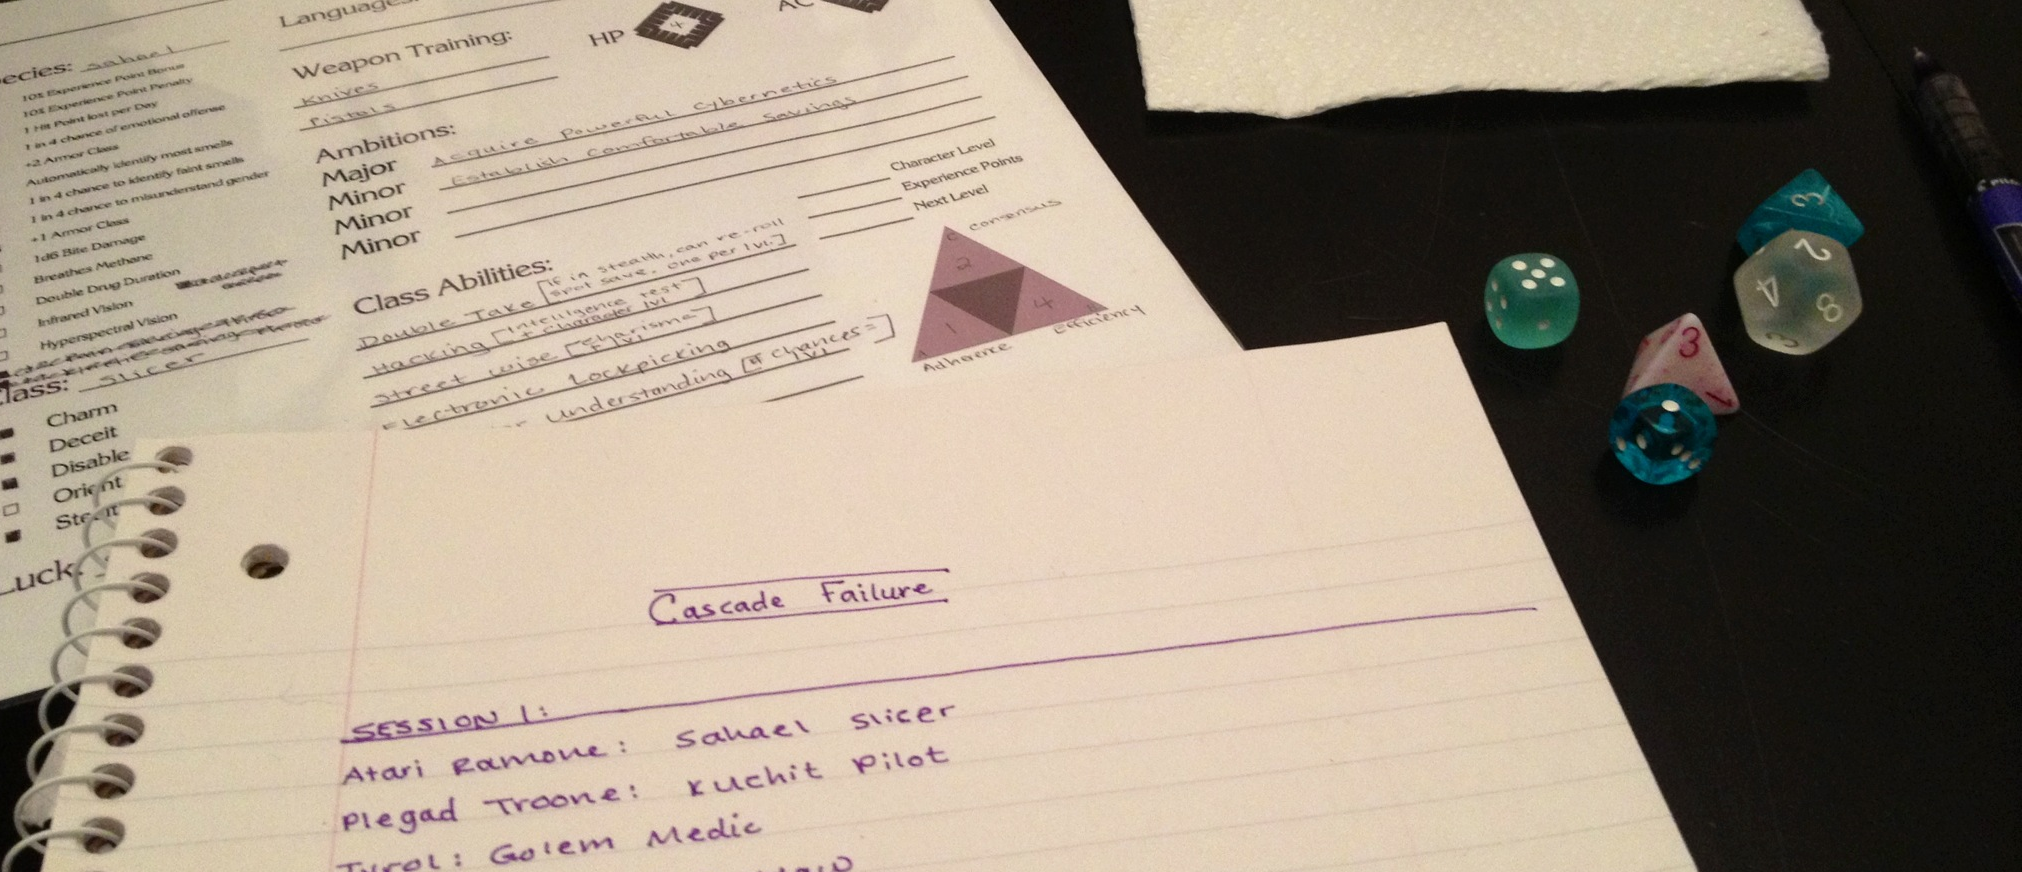
\includegraphics[width=1.00\textwidth]{media/pnp_supplies.png}
	\caption [Typische Ausrüstung bei einer PnP-Spielrunde: Würfel, Notizen und Charakterbogen.]{Typische Ausrüstung bei einer PnP-Spielrunde: Würfel, Notizen und Charakterbogen.\protect\footnotemark[1]}
	\label{fig:pnp_supplies}
	 \footnotetext[1]{http://eclectickellycole.wordpress.com, 20.03.14 }
		 \end{minipage}
\end{figure}

Pen-\&-Paper-Rollenspiele (im folgenden auch als PnP bezeichnet) stellen eine Urform des Rollenspiels dar \cite{Apperley2006}. Mehrere Spieler treffen sich um gemeinsam ein Abenteuer zu erspielen. Einer der Spieler nimmt dabei die Rolle des Spielleiters ein. Die Spieler werden von dem Spielleiter durch ein fiktives Abenteuer geführt, wobei in der Regel der genaue Verlauf der Geschichte stark von der Interaktion der Mitspieler abhängt. \cite{Apperley2006}\newline 
Eine Besonderheit von PnP-Rollenspielen ist, dass keinerlei reales Rollenspiel stattfindet. Zwar erhalten die Spieler oftmals begleitende Materialien wie etwa Karten vom Spielleiter, das eigentliche Spiel findet jedoch in der Phantasie der Spieler statt \cite{Copier2005}. Die Interaktion mit der Spielwelt erfolgt verbal, Spieler treffen Aussagen über Aktionen die der Charakter ausführen soll. Der Spielleiter validiert diese Aussagen und antwortet mit dem Resultat der Aktion. Durch diese Art der Kommunikation ergibt sich oftmals ein dynamischen Abenteuer, welches speziell auf die Spielergruppe zugeschnitten ist. \cite{Drachen2008}\newline
Eines der ältesten und wohl auch bekanntesten PnP-Regelsysteme ist das 1974 vorgestellte \emph{Dungeons \& Dragons} (kurz \emph{D\&D}). Dieses Regelsystem vereint die damals sehr populären \emph{Wargames} mit dem literarischen Fantasy-Genre. \cite{Copier2005}


\subsection{Spielleiter}
\label{sec:Spielleiter}
%Beschreibung der Tätigkeiten und Funktion von Spielleitern beim PnP\newline
%Abdecken von:
%\begin{itemize}
%	\item Konzeption und Umsetzung eines Abenteuers ('offline' vor der Spielrunde)
%	\item Durchführen des Spieles ('online' währen der Runde mit dem Spielern zusammen)
%\end{itemize}
Der Spielleiter hat bei einem PnP-Rollenspiel die Aufgabe eine Geschichte für die Spielrunde zu erdenken und die Teilnehmer während des Verlaufes anzuleiten. Im Vorfeld der Spielrunde konzipiert der Spielleiter dafür in der Regel eine Ausarbeitung eines Abenteuers. Meist werden hierfür Kerncharaktere und wichtige Entscheidungspunkte und Szenen ausgearbeitet, während sich der genaue Verlauf des Abenteuers beim Spielen ergibt. \ref{fig:storyflow_pnp} zeigt, wie sich aus mehreren Ideen des Spielleiters durch Einflussnahme und Interaktion der Spieler eine Geschichte ergibt. Das Bild veranschaulicht, wie der Spielleiter verschiedene Eckpunkte ausgearbeitet hat (D1-En) welche durch die Interaktionen der Spieler und Geschehnisse wahrgenommen, oder verworfen werden und somit die erlebte Geschichte ergeben (A, B und C). Um diese Entwicklung zu ermöglichen muss der Spielleiter verschiedene Funktionen erfüllen.\newline
\cite{Arinbjarnar} nennt drei verschiedene Kernaufgaben des Spielleiters: \emph{Storyteller}, \emph{Actor} und \emph{Judge}. Zum einen ist es die Aufgabe des Spielleiters die Geschichte aus objektiver Sicht zu erzählen und die Handlung mit den Spielern voranzutreiben. Gleichzeitig nimmt er jedoch auch die Rolle und den Standpunkt aller NSCs ein und vermittelt zwischen ihnen und den Spielern. Als letzte Aufgabe achtet der Spielleiter auf die Einhaltung aller Regeln und trifft Entscheidungen falls es zu Unstimmigkeiten kommt.
\begin{figure}
	\centering
		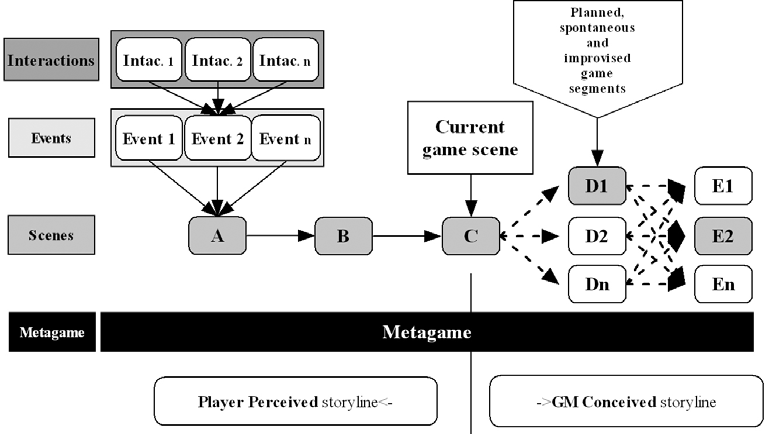
\includegraphics[width=1.00\textwidth]{media/storyflow_pnp.png}
	\caption{Entwicklung eines Pen-\&-Paper-Abenteuers im Verlauf der Spielrunde nach \cite{Tychsen2006a}}
	\label{fig:storyflow_pnp}
\end{figure}


\subsection{Spielermotivation}
\label{sec:Spielermotivation}

%\begin{itemize}
%	\item Hervorheben was die PnP Spieler wollen (nach Möglichkeit belegen: Paper, Foren, unsere Testspieler, Pathfinder Entwickler)
	%	\begin{itemize}
%		\item Kreative Interaktive Geschichte
%		\item Soziale Komponente
%		\item 'Gemeinsam Abenteuer erleben'
%	\end{itemize}
%\end{itemize}
Im Gegensatz zu digitalen Rollenspielen geht es den Spielern von PnP-Rollenspielen meist weniger um die Charakterprogression oder das Absolvieren von \emph{Quests}, sondern um das gemeinsame Erleben einer interaktiven Geschichte. Die Geschichte kann durch Entscheidungen von Spielern aktiv mitgestaltet werden indem sie durch Rollenspiel die von dem Spielleiter vorgestellten Szenarien ausfüllen. Eine Spielergruppe kann so den Pfad eines Abenteuers relativ frei ausgestalten. Zwar ist die Geschichte in Grundzügen geplant, aber die Spieler entscheiden sich immer wieder aufs Neue welchen Weg sie wählen möchten. \cite{Arinbjarnar}\\
Die Freiheit, eigene, nicht standardisierte Handlungen umsetzen zu lassen und in der Gruppe auf die teils unvorhersehbaren Konsequenzen zu reagieren stellt den Reiz von PnP-Spielen dar. 


\subsection{Gängige Spielmechaniken}
\label{sec:Spielmechaniken}

In den meisten PnP-Regelwerken ist es üblich viele Aktionen mit einem Zufallsfaktor zu versehen. Dazu werden Würfel unterschiedlicher Größenordnung und Anzahl verwendet. Ein Würfel mit 6 Seiten wird durch \textit{W6} abgekürzt, weitere Würfel sind zum Beispiel \textit{W2} (eine Münze), \textit{W4}, \textit{W8}, \textit{W10}, \textit{W12} und \textit{W20}.\newline
Charaktere besitzen überdies Fähigkeiten deren Werte mit denen eines Würfelwurfes verrechnet werden und den Ausgang einer Aktion beeinflussen. Das Ergebnis einer Rechnung wird dann mit einem durch andere Charaktere berechneten oder vom Regelwerk oder Spielleiter festgelegten Wert verglichen. Dieses Vorgehen wird als Probe bezeichnet und kann einen erfolgreichen, wirkungslosen oder fatalen Ausgang nehmen.\newline
Für besonders gelungene Spielzüge kann der Spielleiter Erfahrung verteilen. Je nach Spielweise werden zusätzlich Ressourcen und Lehrer benötigt um mit diesen Punkten Fähigkeiten zu steigern und damit den Charakter zu entwickeln. Dadurch können Proben besser absolviert oder erst ermöglicht werden.

Eine Besonderheit von PnP Spielen im Vergleich zu digitalen Rollenspielen ist, dass sie auf keine allgemeingültige Repräsentation der Spielwelt zurückgreifen können. Das eigentliche Spiel findet nur in der Fantasie der Spieler statt. Daher ist die Kommunikation zwischen den Spielern ein wichtiges Instrument um das eigenen Verständnis der Spielwelt abzugleichen und um geplante Aktionen an den Spielleiter weiterzugeben.\cite{Drachen2008}

\section{Digitale Rollenspiele}
\label{sec:DigitaleRollenspiele}
%
%Beschreibung eines Standard Pc-Rollenspiels mit Mechaniken und Möglichkeiten\newline
%Dient später der Abgrenzung zu unserem Prototypen
%\begin{itemize}
%	\item DSA Reihe
%	\item D\&D Online
%	\item Neverwinter Nights
%	\item Elder Scrolls
%	\item Baldurs Gate
%	\item Icewind Dale
%\end{itemize}
%Besonders auf die D\&D basierten eingehen, den rest nur als Beispiele für andere Systeme.

Digitale Rollenspiele basieren häufig auf einem ähnlichen Regelwerk wie Pen-\&-Paper-Spiele. Die exakten Formeln werden in ein festes Regelwerk überführt, welches der Computer zur Evaluierung aller Werte und Möglichkeiten nutzen kann. Anders als bei PnP-Spielen wir den digitalen Spielen jedoch ein starker Fokus auf die visuelle Repräsentation gelegt \cite{Tychsen2006}. Diese visuelle Repräsentation ersetzt die imaginäre Spielwelt von PnP-Rollenspielen. Dadurch ist keine kontinuierliche Kommunikation und Synchronisation von Ereignissen und Umgebungen zwischen Spielleiter und Spielern mehr nötig \cite{Drachen2008}.\newline
Gleichzeitig geht ein Großteil der Kontrolle über den Spielverlauf vom Spieler an den Computer über. Der Spieler muss, anders als bei PnP-Spielen, nicht zwingend Verständnis über die Regeln des Spieles haben. Alle Entscheidungen werden im Hintergrund durch den Computer getroffen und in der visuellen Repräsentation reflektiert. Dieses strikte Vorgehen verhindert das variieren von Regeln. Während ein PnP-Spielleiter kreative Entscheidungen auf Basis der bekannten Regeln treffen kann, ist der Computer an exakt den vordefinierten Regelsatz gebunden. \cite{Drachen2008}

Als Beispiel sei das Rollenspiel \emph{Neverwinter Nights}\footnote{http://de.wikipedia.org/wiki/Neverwinter\_Nights} genannt, welches auf dem D\&D-Regelwerk der 3. Edition basiert. Mit der AURORA Engine ist es möglich ein eigenes Abenteuer zu erstellen und mit anderen Spielern über das Netzwerk zu spielen. Sogar rudimentäre Spielleiter-Tools sind vorhanden. Allerdings kann kein Spieler jemals das Regelsystem des Spieles verlassen und eine Aktion ausführen, welche nicht von den Entwicklern implementiert wurde.\cite{Tychsen2006a}



\section{Bestehende Ansätze}
\label{sec:BekannteAnsaetze}
%Paper und Programme die unserem Thema ähneln, jeweils mit Abgrenzung warum sie die Frage nicht zufriedenstellend (oder wenigstens schlechter als wir) beantworten können
%\begin{itemize}
%	\item RPG Maker
%	\item NWN
%	\item GM-AI
%	\item Tools die ähnliches leisten
%\end{itemize}

Das in \ref{sec:DigitaleRollenspiele} genannte \emph{Neverwinter Nights} wird mit einem Editor und einem Spielleiter-Tool ausgeliefert, welche das Erstellen und leiten eigener Abenteuer erlauben. Hierbei werden dem Spielleiter erweiterte Möglichkeiten in der Spielwelt zugesprochen, allerdings ist der Spielleiter dabei stets an die im Spiel implementierten Regeln gebunden. \cite{Tychsen2006a}\newline
Auch Tools die spezifisch zum Erstellen kleiner Rollenspiele entwickelt wurden wie der \emph{RPG Maker} \footnote{http://www.rpgmakerweb.com/} erreichen nicht die Handlungsfreiheit von PnP-Rollenspielen. Der RPG Maker erlaubt es dem Entwickler~/~Spielleiter neue Objekte zu erstellen und mit eigener Logik zu versehen. Nach der Distribution des RPGs ist der Spieler jedoch wiederum an das erdachte Regelsystem gebunden eine wirkliche Interaktion des Spielers und der Regelwelt des RPGs ist nicht möglich.\newline
Die meisten aktuell vorhanden Tool leiden unter dem Problem das die in \cite{Arinbjarnar} beschriebene dynamische Entwicklung der Geschichte nicht während des Spiels stattfinden kann. Eigene Regelsysteme und Questslinien müssen zumeist vor dem Abenteuer ausgearbeitet und finalisiert werden und während des Abenteuers hat die Spielergruppe nur marginalen Einfluss auf die Auslegung verschiedener Mechaniken.\newline
In der Forschung finden sich auch Ansätze um die Funktion eines Spielleiters durch ein Computersystem wahrnehmen zu lassen. \cite{Aylett2007} vergleicht die Arbeitsweise eines Spielleiters mit Problemen aus der Robotik. Aus vordefinierten Mustern müssen unter Berücksichtigung sich wechselnder Umwelteinflüsse die eigentlichen Handlungen konstruiert werden. Die Eckpunkte stellen im PnP-Kontext die vorher geplanten Geschichts-Eckpunkte dar, die Spielerentscheidungen während der Runde sind die äußeren, nicht planbaren Einflüsse.\newline
Diese \emph{digitalen Spielleiter} erzeugen Geschichten, Quests und Aktionen aus verschiedenen abstakten Regeln und sind damit in der Lage auf Entscheidungen der Spieler zu reagieren. \cite{Arinbjarnarb} gibt eine umfassende Übersicht über verschiedene Systeme dieser Art. Als Beispiel sei hier \emph{Directed Emergent Drama} (kurz \emph{DED}) \cite{Arinbjarnara} genannt, eine Spielform, in der einzelne Akteure von einem zentralen Programm angeleitet werden. DEDs nutzen so genannte Schemata um Charakteren verschiedene Rollen zuzuordnen. Je nach Zustand des Dramas vergibt der Regisseur verschiedene Schemata an die Akteure um die Geschichte voranzutreiben \cite{Arinbjarnarb}. Die Handlungen der Akteure und Spieler werden im Rahmen der zugeordneten Schemata analysiert und bei zu großen Abweichungen des aktuellen Schemas wird dieses von dem Direktor durch ein passenderes ersetzt \cite{Arinbjarnar}.\newline
Während dieser Ansatz eine dynamischere Reaktion auf Aktionen der Spieler ermöglicht ist die künstliche Intelligenz immer noch auf ihren Regelsatz beschränkt. Die Kreativität eines menschlichen Spielleiters, welche es erlaubt die Spielwelt während des Spiels konstant anzupassen würde von dem Computer eine andauernde Evaluierung der Spieler-Aktionen und Umgestaltung der Spielwelt erfordern.\newline
Der in diesem Paper konzipierte Prototyp behandelt diese Probleme indem er dem Spielleiter die Möglichkeit gibt alle Objekte und ihre Eigenschaften zur Spielzeit frei zu manipulieren. Dies erlaubt es Spielern eigene, kreative Ideen in das Spiel einzubringen und dem Spielleiter diese Vorschläge bei Bedarf in das Spielsystem einzupassen. So erwächst bei jeder Spielrunde eine dynamische Spielwelt, welches den Anforderungen der Gruppe und des Abenteuers genügt.

\chapter{Konzept}
\label{concept}
In den Abschnitten dieses Kapitels werden verschiedenen elementare Konzepte vorgestellt, welche im Prototypen zum Einsatz kommen. Nach einer Übersicht über das Grobkonzept werden Kernelemente und interaktive System erläutert um abschließend in \ref{sec:Spielfluss} das Zusammenspiel der einzelnen Systeme an einem kurzen fingierten Abenteuer aufzuzeigen.

\section{Spielkonzept}
\label{sec:Grobkonzept}
%\emph{Beschreibung des generellen Prototypen. Auf keinen Fall technisch.}
Der zur Beantwortung der Frage umgesetzte Prototyp benutzt eine abstrakte, zwei-dimensionale Darstellung um eine rudimentäre visuelle Repräsentation des Abenteuers bereit zu stellen. Diese abstrakte Darstellung wurde bewusst gewählt um die Spieler dazu anzuregen weiterhin eine eigenen Vorstellung der bespielten Welt zu pflegen. Mehrere Spieler~(Clients) verbinden sich mit einer Spielleiter-Instanz~(Server) über das Internet oder ein lokales Netzwerk. Der Prototyp implementiert verschiedene Komponenten welche das Durchführen einer PnP-Spielrunde mit dem analogen Original ähnlicher Stimmung und Spielfluss erlaubt.



\subsection{Kernelemente}

%\begin{itemize}
%	\item Abstrakte Tile based world
%	\item Spielleiter kann Welt/jedes Objekt editieren
%	\item Spieler haben Echtzeit Rollenspiel + rundenbasierten Kampfmodus
%	\item Annahme: TeamSpeak oder ähnliche effective Kommunikation
%	\item Clienten (Spieler),  Server (GM)
%	\item Objectsystem, Rechtesystem
%\end{itemize}

\begin{figure}
	\centering
		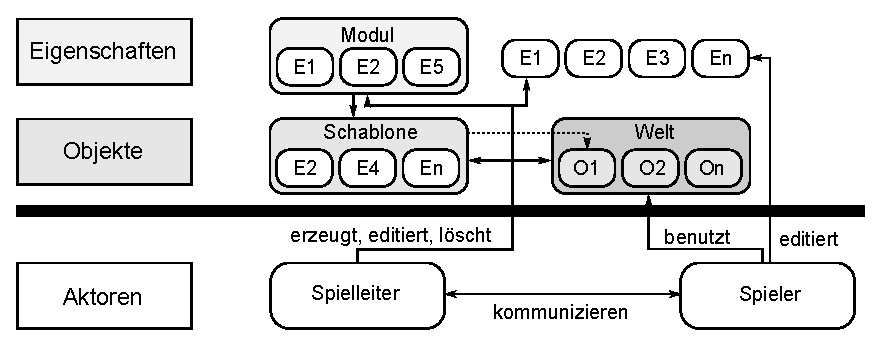
\includegraphics[width=1.00\textwidth]{media/konzept_schema.eps}
	\caption{Schematische Darstellung der komponentenbasierten Welt, Aktionen hängen nur von der Existenz und den Werten der Eigenschaften ab.}
	\label{fig:konzept_schema}
\end{figure}

Hauptkomponente des Prototypen ist ein frei definierbares Objektsystem. Zu jedem Zeitpunkt steht es dem Spielleiter frei Objekte und Werte derartig zu verändern, dass ein völlig anderes Vorgehen ermöglicht wird. Intern behandelt der Prototyp alle Elemente als gleichwertige Objekte. Diesen Objekten können verschiedene Eigenschaften zugeordnet werden, welche das Verhalten der Objekte definieren. Dieses System erlaubt es dem Spielleiter jedes Objekt in der Spielwelt zu editieren und bei Bedarf mit weiteren Daten anzureichern. Schlägt ein Spieler vor einen Gegenstand aus der Umgebung als Waffe zu nutzen, so kann der Spielleiter dem entsprechenden Objekt einen Schadenswert hinzufügen und diesen später in der Berechnung des Kampfwertes nutzen.\newline
Durch Module und Schablonen werden dem Spielleiter vorgefertigte Kombinationen von Eigenschaften und direkt verwendbare Objekte geliefert, welche er bei Bedarf schnell einsetzen kann. Mit dieser Option kann er das Verhalten der Spielwelt schnell ändern, was die Einwirkung bei laufendem Spiel ermöglicht.\newline
Ein internes Rechtesystem erlaubt es Spielern nur einen gewissen Teils dieser Eigenschaften zu sehen oder diese ändern zu können. Auf diese Weise kann er zwar z.B. seine Trefferpunkte selbst verwalten, aber keine beliebigen Gegenstände verändern.
%NEE KANN ER LEIDER NICHT (gibt keine gui dafür). Über ein internes Rechtesystem kann der Spielleiter zudem definieren in welcher Weise die Objektdaten für Spieler sichtbar sind. So kann zum Beispiel einem Waldläufer eine Eigenschaft, die Daten über eine Fährte enthält, angezeigt werden, anderen Spielern bleibt diese Information jedoch verwehrt. Dies erlaubt es dem Spielleiter gezielt Daten für einzelne Spieler frei zu geben, oder aber auch Objekte wie NPCs oder Items mit Notizen anreichern, die nur für ihn selbst sichtbar sind.\newline
Der Prototyp liefert in einer Anwendung eine Server- und eine Clientansicht aus. Der Spielleiter kann die Serveransicht nutzen um vor der Spielrunde das Abenteuer zu erstellen und leitet aus dieser Sicht heraus auch den Spielverlauf. Sobald der Server aktiviert wurde können sich die Spieler mit ihm verbinden und starten damit die Clientansicht. Um eine ähnlich flüssige Kommunikation wie bei analogen PnP-Runden zu ermöglichen wird davon ausgegangen, dass ein Echtzeitkommunikationsmedium wie z.B. Teamspeak\footnote{http://www.teamspeak.com/} oder Skype\footnote{http://www.skype.com/} genutzt wird. Zusätzlich bietet der Client noch einen einfachen Chat, über den Statusmeldungen, Spielernachrichten und verbal beschriebene Aktionen der Spielfiguren ausgegeben werden können. \newline
Die Interaktion der Spieler mit der Spielwelt geschieht in Echtzeit. Während eines Kampfes wechselt der Prototyp in das typische rundenbasierte Kampfsystem, welches auf den D\&D-Regelsystem basiert. Dem Spielleiter stehen gleichzeitig alle Optionen offen die Spielwelt im laufenden Spiel zu editieren.\newline
Durch die Kombination des offenen Objektsystems und der abstrakten Darstellung, welche schnell verändert oder durch eigene Grafiken erweitert werden kann, bietet der Prototyp damit ein Hilfsmittel um eigene, persönliche Abenteuer zu erstellen und in einer PnP-Runde zu durchspielen.


\section{Interaktive Systeme}
\label{sec:InteraktiveSysteme}
Ein System veränderbarer Objekte erschafft zwar einen Baukasten, aber ein Spielfluss wird dadurch noch nicht realisiert. Das folgende Nachrichtensystem ist so allgemein gehalten, dass sich viele Aktionen direkt damit realisieren lassen. Das zusätzliche Kampfsystem setzt den häufig zentralen Teil des Kämpfens auf Basis des D\&D-Regelwerkes um.

\subsection{Kampfsystem}
\label{sec:Kampfsystem}
Ein großer Teil des D\&D-Regelwerkes befasst sich mit dem Ablauf von Kämpfen. Um den Aufwand überschaubar zu halten finden im Rahmen dieser Ausarbeitung nur die wichtigsten Regeln Beachtung. Diese Regeln werden im Folgenden kurz erklärt.~\cite{SRD35}

Der Kampf in D\&D läuft in Runden ab. Zu Beginn eines Kampfes machen alle Teilnehmer einen Initiativewurf, d.h. einen Wurf mit einem W20 auf den der u.a. von der Geschicklichkeit des Charakters abhängige Initiative-Modifikator addiert wird. Die Ergebnisse der Initiativewürfe bestimmen die Kampfreihenfolge, der Teilnehmer mit dem höchsten Initiativewert beginnt.\\
Die Runde eines Kampfteilnehmers besteht aus zwei großen Aktionsblöcken: \emph{Standardaktion} und \emph{Bewegungsaktion}. Mit der Standardaktion kann der Charakter jede Aktion ausführen, die im Regelbuch oder vom Spielleiter als solche deklariert wird. Dies sind z.B. ein einfacher Angriff oder das Wirken bestimmter Zauber. Die Bewegungsaktion erlaubt die Bewegung des Charakters über eine Distanz die nicht höher ist als seine Bewegungsrate. Dieser Wert hängt von der Rasse, Ausrüstung und anderen Faktoren des Charakters ab. Weiterhin kann die Bewegungsaktion durch eine bewegungsentsprechende Aktion ersetzt werden, z.B. das Laden einer schweren Armbrust oder das Aufstehen aus dem Liegen.\\
Aktionen, die eine komplette Runde in Anspruch nehmen (also Standard- und Bewegunsaktion verbrauchen) heißen \emph{Volle %SIC: im Regelbuch als Eigenname verwendet!
Aktion}. Eine häufig verwendete Aktion dieser Art ist der \emph{Volle Angriff}, bei dem mehrere Angriffsaktionen in einer Runde ausgeführt werden können.\\
Findet in der Runde keine tatsächliche Bewegung statt und verbietet keine der verwendeten Aktionen dies, so steht dem Teilnehmer ein 1,5m-Schritt zu.\\
Darüber hinaus gibt es weitere Aktionen, die keine oder sehr wenig Zeit in der Runde einnehmen und somit nach Ermessen des Spielleiters zusätzlich ausgeführt werden können. Diese Aktionen heißen \emph{Freie Aktion} oder \emph{Keine Aktion}.

Führt ein Kampfteilnehmer einen Angriff aus, so werden möglicherweise mehrere Würfe von ihm verlangt. Der erste Wurf heißt \emph{Angriffswurf} und bestimmt ob das Ziel getroffen wird oder nicht. Der Angriffswurf besteht immer aus einem W20. In der Regel wird Grundangriffsbonus des Charakters addiert, bei Nahkampfangriffen zusätzlich der Stärke- und bei Fernkampfangriffen der Geschicklichkeits-Modifikator. Eine \emph{natürliche 1} (dies bedeutet, dass der W20 nur ein Auge zeigt) führt nie zu einem Treffer, während eine \emph{natürliche 20} immer trifft. Ansonsten trifft der Angriff, falls das Ergebnis des Angriffswurfs mindestens so hoch ist wie die von Geschicklichkeits-Modifikator, Ausrüstung und weiteren Faktoren abhängige Rüstungsklasse des Ziels.\\
%Abhängig von der zum Angriff verwendeten Waffe können hohe Augenzahlen des W20 zu einem kritischen Treffer führen. Hierfür ist ein erneuter Angriffswurf durchzuführen, für dessen Evaluation die gleichen Regeln gelten. Trifft dieser Angriff (auch durch natürliche 20), so gilt der Treffer als kritisch und der Schaden wird, wiederum abhängig von der Waffe, mehrfach ausgewürfelt. \todo{Haben wir nicht implementiert, ist mir leider erst nach dem Schreiben aufgefallen. Evtl. trotzdem rein?}\\
Bei einem erfolgreichen Angriff wird vom Angreifer ein \emph{Trefferwurf} ausgeführt. Dieser bestimmt wie viel Schaden das Ziel nimmt. Abhängig von der Waffe wird ein bestimmter Würfel verwendet. Bei Nahkampfangriffen wird in der Regel der Stärke-Modifikator addiert, bei anderen Angriffen gelten andere Regeln. Das Ergebnis des Wurfes ist stets mindestens 1, selbst wenn ein Malus addiert wird. Der ermittelte Wert wird dann, nach eventuellem Abzug von Schadensreduzierung durch spezielle Fähigkeiten des Ziels, von den Trefferpunkten (TP) des Ziels abgezogen. Sinken die TP des getroffenen Teilnehmers unter 0, so ist er ohnmächtig und kann nicht mehr agieren. Bei -10 Lebenspunkten ist der Charakter tot.

Für die genannten Regeln enthält der Prototyp ein Kampfsystem, welches den Ablauf steuert und die genannten Würfe verlangt. Über diese Regeln hinaus wurde bei der Konzeption des Prototypen darauf geachtet, dass auch andere Aktionen durch manuelles Eingreifen des Spielleiters möglich sind und nicht vom System unterbunden werden. Weiterhin wurde darauf geachtet, dass die Freiheit des Spielleiters nicht eingeschränkt wird. Sinken z.B. die TP eines Charakters durch Würfelglück eines Spielers unter -10 möchte der SL den getroffenen Charakter jedoch möglicherweise weiterkämpfen lassen, da ihm der Kampf zu einfach schien. Die Entscheidung den Charakter zu töten und zu entfernen wird also nicht automatisch vom System getroffen sondern liegt ultimativ beim SL.




\subsection{Nachrichtensystem}
\label{sec:Nachrichtensystem}
Während der Prototyp nicht auf ein Echtzeitkommunikationsmedium wie z.B. Teamspeak verzichten kann bietet er mit seinem Nachrichtensystem eine zusätzliche Mechanik an um den Informationsfluss im Spiel zu steuern. 
Über den Chat lassen sich Nachrichten und auch einfache \emph{Emotes} versenden. Dies soll im Spiel eine gewissen Form des Rollenspiels ermöglichen um zum Beispiel Gefühlsregungen des Charakters zum Ausdruck zu bringen, während ein anderer Teilnehmer gerade spricht. Verschiedene Ereignisse wie Würfelergebnisse oder das Auslösen eines Schalters werden ebenso im Chat ausgegeben wie Fehler in eingegebenen Formeln. Der Chat dient damit neben der Kommunikationsfunktion auch als Protokoll für das Abenteuer.\newline
Zusätzlich zum Chat können verschiedene Aktionen von Spielern oder vom Spielleiter gefordert werden, zum Beispiel das Auswürfeln der Initiative zum Kampfbeginn. Solche angeforderten Aktionen werden mit ihrem jeweiligen Symbol am unteren Bildschirmrand angezeigt und können minimiert, bzw. aufgeklappt werden.\newline
Eine wichtige Aktion dieser Art ist die \emph{Freitextaktion}, welche von einem Spieler auf ein beliebiges Objekt angewendet werden kann. Der Spielleiter erhält daraufhin eine solche Meldung mit dem Ausführenden und dem Ziel der Aktion, sowie dem vom Spieler eingegebenen Freitext. Der Spielleiter hat dann direkt in der Nachricht die Möglichkeit zu den betroffenen Objekte zu springen um die Situation zu analysieren und entsprechend zu entscheiden.


\section{Spielfluss}
\label{sec:Spielfluss}
%Wird vermutlich eines der größten Kapitel im Konzept werden. Anhand der vorherigen Abschnitte erklären wie eine 'Spielsession' aus Sicht der Spieler und des Spielleiters ablaufen würde. Daran werden die Entscheidungen aus den vorherigen Abschnitten gerechtfertigt.\newline
%\todo{Überlegen ob wir das in einem Kapitel machen und Spieler / Spielleiter optisch abgrenzen können (Vorteil es ist zeitlich synchron, aber evtl. anstrengender zu lesen) oder ob wir in Spieler / Spielleiter Unterkapitel trennen (Hier wäre ganz kalr worum es grade geht, aber Ereignisse sind nicht mehr synchron. Alles in einem Fluss, verschiedene Schriftarten/Farben möglich; Auf jeden fall sehr deutlich. \textbf{Möglickeit: Logische Kapitel und dann Spielleiter/Spieler getrennt.}}

In diesem Kapitel wird die Funktionsweise und das Zusammenspiel der verschiedenen vorgestellten Systeme anhand eines kurzen Abenteuers aus Sicht der Spieler und des Spielleiters erläutert.\newline
Der Spielleiter, im folgenden auch \emph{SL} genannt, beginnt damit ein Abenteuer zu konzipieren und vor zu bereiten. In diesem Szenario sollen die Spieler in einer Taverne von dem Wirt beauftragt werden seltsamen Geräuschen aus dem Keller nachzugehen. Im Keller finden die Spieler einen Durchbruch in ein tieferes Gewölbe und müssen sich dort dem Kampf mit zwei Goblins stellen, um am Ende mit einer Schatztruhe belohnt zu werden.\newline

\subsection{Vorbereitung}
\label{sec:Vorbereitung}
Der SL beginnt seine Vorbereite mit dem Layout der Umgebung. Dafür greift er auf verschiedene generische Tiles zu und nutzt die frei-definierbare Farbe um diverse Materialien darzustellen. Mit diesen Tiles erstellt er zwei verschiedene Karten, die Taverne und das Gewölbe, welches aus einem Eingangsbereich und einem größeren Raum für den Kampf und die Truhe besteht. Für die Gegner könnte der Spielleiter eine der vorbereiteten Schablonen nutzen, er entscheidet sich jedoch dafür einen eigenen Gegnertyp zu definieren. Dafür erstellt er ein neues Objekt und weist ihm eine Grafik zu. Danach fügt er das \emph{'Angreifbar'} Modul hinzu, welches die Eigenschaften \emph{'Trefferpunkte'} und \emph{'Rüstungsklasse'} enthält. Die Rüstungsklasse setzt der SL auf den fixen Wert 12 und die Trefferpunkte auf 15.\newline
Der SL platziert nun zwei Instanzen der grade erstellen Vorlage und eine Instanz der Truhen-Schablone in dem Verlies. Die Truhe besitzt eine Inventar Eigenschaft, die der Spielleiter nun mit einigen Münzen und einem Rüstungsobjekt befüllt. Zuletzt versiegelt der SL den Durchgang vom ersten in den zweiten Raum mit einigen bunten Balken, welche als Bücherregal fungieren werden. Einem Regal weißt der Spielleiter das 'Schalter' Modul zu, welches Spielern später die Möglichkeit der Interaktion gibt.\newline
Die Taverne füllt der Spielleitern mit einigen NPCs und Objekten, außerdem platziert er das Modul \emph{Sprungmarke} auf einer Tür im hinteren Bereich der Taverne und verbindet das Sprungziel mit dem ersten Raum der Gewölbe Karte.\newline
Die Vorbereitung des Abenteuers ist hiermit abgeschlossen.

\subsection{Einführung in das Abenteuer}
\label{sec:EinführungInDasAbenteuer}


Zur Spielrunde finden sich neben dem Spielleiter noch zwei Spieler (S1 und S2) ein. Nachdem beide Spieler mit einem an \emph{Pathfinder}\footnote{http://paizo.com/pathfinder}, eine Variante des D\&D-Regelwerkes, angelehnten Charakterbogen die Werte ihres Charakters definiert haben verbinden sie sich mit dem SL-Server. Der Prototyp synchronisiert nun die Spielwelt, Objektvorlagen und Medien des Spiels. Nachdem beide Spieler die Verbindung hergestellt haben platziert der Spielleiter sie in der Taverne.\newline
Die Spieler erkunden die Umgebung und bald entfaltet sich das Rollenspiel. 

\subsection{Rollenspiel}
\label{sec:Rollenspiel}

S1 fordert einen vom SL als besonders düster aussehend beschriebenen NPC zu einer Runde Armdrücken auf.\newline
Der Spielleiter würfelt verdeckt einen Wert für den NPC und fordert S1 auf ebenfalls einen Wurf mit einem W20 zuzüglich es Stärke-Modifikators auszuführen. Diese Eigenschaft ist an das Spielerobjekt angehängt und wird aus den Werten der Attribut Eigenschaften errechnet. S1 merkt an das ihr Charakter eine hübsche, verschlagene Diebin ist und möchte gerne ebenfalls den Charisma-Modifikator mit einbringen. Der SL genehmigt dies und S1 würfelt endgültig mit \emph{'W20 + ST-Mod + }'\emph{CH-Mod}'\emph{'}\newline
S1 gewinnt diesen Wurf und als Preis erhält sie eine Runde Getränke aufs Haus.\newline
Nach einigen Getränken und Gesprächen mit den NPCs, welche der SL über Teamspeak durchführt entscheiden sich die Spieler mit dem Abenteuer fortzuschreiten. 

\subsection{Das erste Rätsel}
\label{sec:DasErsteRätsel}

In einem Gespräch mit dem Inhaber erfahren S1 und S2 das es sonderbare Begebenheit im Keller der Taverne gibt. Der Spielleiter bewegt den Questgeber und gibt den Spielern so den Weg zur vorher definierten Sprungmarke frei.\newline
Voller Tatendrang und beschwingt von den feinen Getränken stürzen sich beide Spieler in das Abenteuer.
Nach der Interaktion mit der Sprungmarke werden beide Spieler automatisch auf der Gewölbekarte platziert. Der Spielleiter beschreibt die Umgebung kurz und lässt die Spieler dann die Umgebung selber erkunden. Bald hat S2 herausgefunden das es die Möglichkeit gibt mit einem der Bücherregale zu interagieren. Der SL erhält die Benachrichtigung darüber über den Chat und entfernt das Bücherregal, während er eindrucksvoll beschreibt wie es sich unter Ächzen und Knarren im Boden versenkt.\newline


\subsection{Der Kampf}
\label{sec:DerKampf}
Die Spieler betreten den zweiten Raum und der Spielleiter fordert sie sofort auf einen Wurf ihre Schleichfähigkeit auszuführen. Das Würfelglück ist nun jedoch nicht bei den Spielern und daher startet sofort ein Kampf mit den Goblins.\newline
Dafür selektiert der Spielleiter die Spieler und die Golbins und startet einen Kampf über seine GUI. S1 und S2 werden dadurch automatisch aufgefordert einen Initiative-Wurf abzulegen, der SL selbst würfelt diesen Wert für die Goblins aus. Es folgen einige Kampfrunden in denen Spieler und Goblins abwechselnd Angriffs und Schadenswürfe sowie Bewegungen ausführen.\newline
Der Kampf siegreich für die Spieler und sie können die Truhe im Raum untersuchen und sich an der reichen Beute bedienen. Der Spielleiter leitet die Spieler nun zurück in die Taverne und erzählt einen kurzen Abschluss des Abenteuers.



\chapter{Implementierung}
\label{implementation}

Auch nicht all zu technisch. Nur grobe Konzepte was wir glauben, wie kritische Parts des GameDesigns umgesetzt werden können.

\section{Objektsystem}
\label{sec:Objektsystem}
Beschreibung unseres Objektsystems\newline


\subsection{Eigenschaften}
\label{sec:Eigenschaften}

\begin{itemize}
	\item Erklärung von Eigenschaften
	\item Beispieleigenschaften mit Funktionalität 
\end{itemize}

\subsection{Rechtesystem}
\label{sec:Rechtesystem}
Beschreibung der Berechtigungen

\subsection{Module}
\label{sec:Module}

\section{Aktionssystem}
\label{sec:Aktionssystem}
Die Existenz von Eigenschaften ermöglicht das Ausführen von Aktionen -> Echtzeitbeeinflussung der Möglichkeiten.

\chapter{Evaluierung}
\label{evaluation}
%Die Beurteilung ist einer der wichtigsten Abschnitte der Arbeit
%- Sie enthält die Quintessenz des gesamten Projektes
%Viele lesen nur die Einführung und die Beurteilung an
%- Hier muss also alles Wichtige drin stehen!
%Hier beweisen Sie dass Sie …
%- die Aufgabe und deren Bedeutung verstanden haben
%- die Ergebnisse richtig zu interpretieren vermögen
%- wissen, worauf es bei diese Arbeit ankam


\section{Erfolgskriterien}
\label{sec:Erfolgskriterien}
Um die Fragestellung zu beantworten wird ein Probandentest mit Teilnehmern, die bereits Erfahrung mit Pen-\&-Paper-Rollenspiel gemacht haben, durchgeführt. Folgende Kriterien dienen am Ende des Projektes zur
Auswertung der Frage:

\begin{enumerate}
	\item Mindestens 66\% der Testspieler fühlen sich in ihrem Handlungsfreiraum nicht eingeschränkt. Im Probandentest soll ermittelt werden, ob Spieler sich subjektiv in ihrem Handlungsfreiraum eingeschränkt fühlen, also ob sie Aktionen ausführen möchten, auf die der Spielleiter nicht reagieren kann.
	\item Höchstens 33\% der Testspieler (inkl. Spielleiter) empfanden die Wartezeiten bei der Umsetzung ihrer Ideen durch den Spielleiter als zu lang. Im Probandentest soll ermittelt werden, ob der Spielleiter auf jede Situation in angemessener Zeit reagieren kann. Dies bedeutet, dass nur wenige Spieler in einer anschließenden Befragung angeben, durch lange Wartezeiten gestört worden zu sein.
	\item Der Spielleiter begreift die Standardfunktionen intuitiv und arbeitet eine Menge von Aktionen in vertretbarer Zeit ab. Der Spielleiter soll in der Lage sein, alle Funktionen, die das Spiel bietet (Objekte erstellen, platzieren, modifizieren, auf Spieleraktionen reagieren etc.), schnell zu begreifen und zu verwenden. Hierfür wird ein Satz von Aufgaben festgelegt, der diese Funktionen beinhaltet. Die Aufgaben müssen innerhalb festgelegter Zeiträume abgeschlossen werden. Die jeweilige Dauer kann der Aufgabenstellung im \hyperlink{AppendixSpielleiter.1}{Testszenario} entnommen werden.
\end{enumerate}

Dieser Probandentest wird über die zwei, im \hyperlink{AppendixFragebogenA.1}{Anhang referenzierten}, Formulare durchgeführt. Das erste Dokument ist ein Fragebogen und wird dabei von allen Teilnehmern ausgefüllt um ein Meinungsbild über verschiedenen Aspekte der Erfolgskriterien zu erhalten. Das zweite Dokument wird speziell von Spielleitern bearbeitet. Es enthält einige Aufgaben die häufiger in der Vorbereitung, bzw. Spielphase einer PnP Runde auftreten. Durch das Messen der benötigten Zeit soll ein Messwert generiert werden, der auf die Arbeitsgeschwindigkeit von Spielleitern schließen lässt.
  



\section{Testaufbau}
\label{sec:Testaufbau}
%\begin{itemize}
%	\item Anzahl der Testspiele
%	\item Anzahl Spieler
%	\item Anzahl unterschiedlicher Spieler / Spielleiter
%	\item Genaue Aufgabenstellung der Tests (Appendix: genau der Fragebogen, den wir rausgeben)
%\end{itemize}
Die Datenerhebung dieser Evaluierung wurde über einen Fragebogen durchgeführt, welcher während eines Probandentest von den Teilnehmern ausgefüllt wurde. Der Fragebogen enthält zehn Fragen, die dazu dienen die Rollenspielerfahrung der Testperson, sowohl digital als auch PnP, zu bestimmen (Frage 1 -3) und ein Qualitätslevel des Prototypen zu evaluieren (Frage 4-10). Die Fragen stellen in allen Fällen Aussagen dar, welche numerisch von 1 bis 4 vom Tester bewertet werden. Folgende Werte wurden dafür festgesetzt:

\begin{enumerate}
	\item Der Tester stimmt der Aussage gar nicht zu
	\item Der Tester stimmt der Aussage eher nicht zu
	\item Der Tester stimmt der Aussage eher zu
	\item Der Tester stimmt der Aussage voll und ganz zu
\end{enumerate}

Die Entscheidung eine Likert Skala\footnote{http://de.wikipedia.org/wiki/Likert-Skala, 18.03.14} mit nur 4 Punkten zu verwenden wurde getroffen, um die Tester zu einer eindeutigen Entscheidung für, oder gegen die Aussage zu zwingen. \cite{Garland1991} hebt hervor, dass bei dem Vorhandensein einer neutralen Option, diese oftmals im Gegensatz zu einer schlechteren Einschätzung zu wählen. In unserem Fall wurden die Tester an die Materie herangeführt und besaßen die nötigen Kenntnisse um die gestellten Aussagen zu bewerten. Die 4 Punkteskala sollte daher eine genauere Entscheidung provozieren ob die betrachteten Feature tatsächlich für die Umsetzung geeignet waren oder nicht.
Die Qualitätsfragen zahlen dabei auf die verschiedenen Erfolgskriterien ein. Mit der genannten Skala bedeutet dies im Detail, dass die Werte 3 und 4 ein erfülltes Erfolgskriterium bedeuten, während 1 und 2 das Erfolgskriterium nicht erfüllen. \newline
Insgesamt wurde die Auswertungen in \todo{Anzahl Testrunden} durchgeführt, wobei \todo{Anzahl Spieler} und \todo{Anzahl Spielleiter} die Fragen ausgefüllt haben. Alle befragten Spieler hatten bereits umfassende Erfahrungen mit PnP Rollenspielen als Spieler und über zwei Drittel haben ebenfalls schon als Spielleiter agiert. Auch bei digitalen Rollenspiele gaben alle Probanden umfassende Kenntnisse an. 



\section{Auswertung}
\label{sec:Auswertung}

In diesem Abschnitt werden die erhobenen Daten in Bezug gesetzt und anhand dieser die Erfolgskriterien evaluiert.

\begin{figure}[h!]
	\centering
		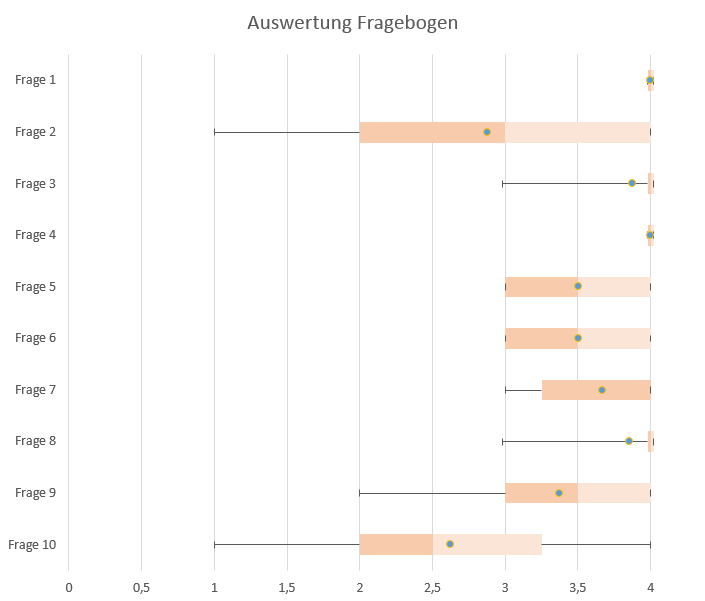
\includegraphics[width=1.00\textwidth]{media/Auswertung.png}
	\caption{Auswertung von Fragebogen A durch Boxplot-Diagramme}
	\label{fig:Auswertung}
\end{figure}



\subsection{Handlungsfreiheit}
\label{sec:Handlungsfreiheit}
Der wohl elementarste Faktor des Prototypen war die Handlungsfreiheit von Spielern und Spielleiter. Dieser Aspekt wird durch die Fragen 4 und 5 auf \emph{Fragebogen A} evaluiert. Zum einen wurde beleuchtet, ob Spieler und Spielleiter sich in der Lage fühlten ihre eigenen Ideen im Spielfluss umzusetzen und damit ihre Kreativen Lösungsstrategien einzubringen, zum anderen wurde ausgeschlossen, dass das Spielsystem den Handlungsfreiraum der Tester einschränkt.\newline
\ref{fig:Auswertung} zeigt die Box-Plot Auswertung dieser Fragen. Der Grafik ist zu entnehmen, dass die Tester während der Probespiels ihre Ideen vollständig umsetzen (Mittelwert: 4) konnten und sich nahezu nicht in ihrer Handlungsfreiheit eingeschränkt fühlen (Mittelwert: 3,5). Insgesamt ergibt sich daher, bei einer Gleichgewichtung beider Fragen ein Durchschnittswert von 3,75. Zur erfolgreichen Erfüllung des Erfolgskriterium müssen mindestens 66\% der Tester sich nicht in der Handlungsfreiheit eingeschränkt fühlen, mit der in \ref{sec:Testaufbau} vorgestellten Skala bedeutet dies, dass 66\% der Tester die Aussagen mit 3 oder 4 bewerten.\newline
Die Auswertung zeigt, dass alle Tester die Fragen mit 3 oder besser bewertet haben. Damit ist gezeigt, dass die Umsetzung eigener Ideen durch den Prototypen möglich ist und Spieler einen Freiraum erfahren, der sonst hauptsächlich aus PnP-Rollenspielen bekannt ist.


	

\subsection{Umsetzungszeit während des Spiels}
\label{sec:Umsetzungszeit}
Um eine Entwicklung der Geschichte und ein immersives Spielgefühl zu ermöglichen darf der Prototyp nicht unverhältnismäßig langsamer sein als die normale Arbeitsweise eines Spielleiters. Benötigt der Spielleiter sehr lange um Aktionen umzusetzen, oder brauchen die Spieler viel Zeit um Werte einzugeben und Aktionen zu formulieren, so wird der Spielfluss gebrochen. Die Fragen 6 und 7 evaluieren daher das zweite Erfolgskriterium, welches fordert, dass die Umsetzungszeit der eigenen Ideen, sowie die Reaktionszeit des Spielleiters in einem annehmbaren Rahmen liegen.
Die \ref{fig:Auswertung} und die \hyperref[fig:tableData]{Datenreihen im Anhang} zeigen, dass auch hier die erhobenen Testdaten alle in dem positiven Bereich liegen\footnote{In den ersten beiden Testrunden war aufgrund der derzeitigen Stabilität des Prototypen keine Beantwortung der Frage 7 möglich}.

Der Prototyp erfüllt damit auch das zweite Erfolgskriterium und erlaubt es Spielern und Spielleitern in einem angemessen Tempo zu agieren und das erdachte Abenteuer zu erfahren.




\subsection{Umsetzungszeit und Bedienung durch den Spielleiter}
\label{sec:UmsetzungszeitUndBedienungDurchDenSpielleiter}
Für das dritte Erfolgskriterium würde im \emph{zweiten Dokument} ein Set von Aufgaben definiert und mit Zeiten versehen. Diese Aufgaben stellen eine Querschnitt der regulären Tätigkeiten eines Spielleiters vor und während einer Spielrunde dar. Im Probandentest wurden die Tester mit Spielleiter-Erfahrung aufgefordert diese Aufgaben abzuarbeiten während die Zeit festgehalten wurde. Der Fragebogen enthält sowohl zeitlich bestimmte Aufgaben, welche das Vorbereiten und Erstellen eines Abenteuers beinhalten, als auch zeitlich unbestimmte Aufgaben welche das eigentliche Rollenspiel darstellen. Die Entscheidung Zweitere ohne zeitlichen Rahmen vorzugeben wurde getroffen, um spontanes Rollenspiel (Wie zum Beispiel Armdrücken in der Taverne) zu ermöglichen. Der flüssige Ablauf dieser zweiten Aufgaben spiegelt sich in Frage 6 und 7 wieder. Im Verlaufe dieses Tests erstellt der SL eine kleine Verlies Karte mit drei Räumen. Raum 1 enthält einen Interaktions-Gegenstand, Raum 2 eine kleine Gruppe Gegner und Raum 3 eine Schatztruhe.\newline
Beim Bespielen beginnt die Gruppe in einer vordefinierten Taverne und wird vom SL durch Rollenspiel in das Verlies geführt wo sie die drei Räume meistern muss. Dieser Test orientiert sich dabei an dem im \ref{sec:Spielfluss} verwendeten Szenario und soll eine breite Übersicht über die Funktionen des Prototypen bieten.\newline
\ref{tab:FragebogenB} zeigt eine Aufschlüsselung der verschiedenen, zeitlich gewichteten, Aufgaben. Dargestellt werden die einzelnen Tätigkeiten, die veranschlagten Zeiten und die im Durchschnitt benötigten Zeiten, diese wurden von dem Testleiter während der Ausführung gemessen. Aus der Tabelle lässt sich entnehmen, dass der SL bei allen Aufgaben schneller arbeiten konnte als veranschlagt wurde. Daraus, in Kombination mit dem zweiten Erfolgskriterium, lässt sich auf eine intuitive Bedienung des Prototypen schließen. Spielleiter konnten ohne große Einarbeitung Funktionen begreifen und schnell eigenen Ideen und Konzepte über die vorgegebenen Arbeitsschritte umsetzen. 
\begin{table}

\begin{tabularx}{\textwidth}{|X|l|l|}
\hline
Aufgabe & Zeit geplant (min) & \O Zeit (min)\\
\hline
\hline
Erstellen einer neuen Karte & 2 & 0.88 \\
\hline
Anlegen von 3 Räumen & 5 & 2 \\
\hline
Erstellen eines Gegners & 3 & 2,8 \\
\hline
Erstellen eines Interaktionsgegenstands & 2 & 1,1 \\
\hline
Platzieren von Gegnern & 1 & 0 \\
\hline
Platzieren und Füllen der Schatztruhe & 2 & 1,5 \\

\hline
\end{tabularx}
\caption{Auswertung vom Spielleiter\-Testszenario}
	\label{tab:FragebogenB}
\end{table}







\chapter{Zusammenfassung}
\label{conclusion}
In dieser Ausarbeitung wurde auf Basis des gängigen Dungeons-\&-Dragons-Regel\-werks ein Konzept erarbeitet, das die Prinzipien des Pen-\&-Papers-Rollenspiels auf digitale Rollenspiele überträgt. Zunächst wurden digitale Rollenspiele mit PnP-Rollenspielen verglichen und die Defizite aufgezeigt. Die Kernelemente von PnP-Rollenspielen wurden identifiziert und während der Erarbeitung des Konzeptes priorisiert.\\

\section{Fazit}
Der konzipierte Prototyp wurde in \ref{sec:Auswertung} anhand der vordefinierten Erfolgskriterien im Probandentest evaluiert. Die Auswertung der Tests ergab, dass alle Erfolgskriterien erfüllt werden konnten. Spieler, die bereits ERfahrungen in PnP- und digitalen Rollenspielen hatten, empfanden die Handlungfreiheit des Prototypen als nicht eingeschränkt. Trotz dieses komplexen und offenen System erlaubt es der Prototyp weiterhin schnell und frei von störenden Verzögerungen zu arbeiten. Spielleiter sind in der Lage nach kurzer Einarbeitung und durch Zuhilfenahme des Handbuches komplexe Probleme eines PnP-Abenteuers in dem Prototypen zu modellieren und zu lösen. Diese Qualität des Prototypen zeigt sich auch in den Fragen 9 und 10 von \emph{Fragebogen A}: Ein Großteil der Tester würde den Prototypen gerne als digitales Hilfsmitteln in privaten PnP-Runden einsetzen. Insbesondere das Kampfsystem, welches durch die abstrakte, leicht zu erstellende Welt und das intuitive Setzen und Bewegen der Figuren ein schnelles und einfaches Hilfsmittel darstellt.
\todo{noch kein ersatz weil zu viele regeln fehlen}


%In dieser Ausarbeitung wurde auf Basis des gängigen Dungeons-\&-Dragons-Regel\-werks ein Konzept erarbeitet, das die Prinzipien des Pen-\&-Papers-Rollenspiels auf digitale Rollenspiele überträgt. Zunächst wurden digitale Rollenspiele mit PnP-Rollenspielen verglichen und die Defizite aufgezeigt. Die Kernelemente von PnP-Rollenspielen wurden identifiziert und während der Erarbeitung des Konzeptes priorisiert.\\
%Anhand eines Prototyps wurde das Konzept umgesetzt und im Probandentest evaluiert. Die Auswertung der Tests ergab zunächst, dass unser Prototyp intuitiv und effizient nutzbar und somit geeignet ist, um die Fragestellung zu beantworten. Weiterhin konnte in den Tests eine erfolgreiche Übertragung der PnP-Prinzipien auf digitale Rollenspiele bestätigt werden. Die Fragestellung, die den Kern dieser Ausarbeitung darstellt, wurde somit bestätigt.

\section{Zukünftige Arbeiten}
\label{sec:futurework}

Der Prototyp konnte zeigen, dass es möglich ist, ein PC-RPG zu erschaffen welches die Handlungsfreiheit der Spieler nicht einschränkt. Ein völlig freies System verliert jedoch oftmals an Komfort, den andere Systeme durch das Treffen gewisser Annahmen gewinnen können. In unserem Konzept wurde dieses Problem dadurch umgangen, dass der Spielleiter stets uneingeschränkt handeln kann und Komfort-Mechanismen wie z.B. das Kampfsystem verwenden \emph{kann}, aber nicht \emph{muss}. Dieser Komfort ist jedoch ein entscheidender Faktor, den digitale Rollenspiele den PnP-Rollenspielen voraus haben. In unserem Prototyp haben wir nur einen Bruchteil der Regeln von Dungeons \& Dragons implementiert. Die Implementierung des kompletten Regelwerks sprengt bei Weitem den Rahmen dieser Ausarbeitung, wäre jedoch nun, da unsere Fragestellung positiv beantwortet werden konnte, ein angemessener nächster Schritt.

\todo{Wir haben konkrete Tickets (Zauber, Objekte größer als 1x1 Tile, Waffenslots und besseres Inventar, mehr Chat-Funktionen) die jedoch alle, wenn man den Text liest, nicht wirklich relevant werden. Trotzdem rein?}

%*********************************************************************%
% APPENDIX                                                            %
%*********************************************************************%

\ifnotdraft{
	\renewcommand*{\firstacronymfont}[1]{\emph{#1}}
	\printglossary[type=acronym,title=List of Acronyms,toctitle=Abkürzungsverzeichnis]
}

\appendix
%\chapter{Anhang}
\label{appedixa}
\begin{figure}[h]
	\centering
		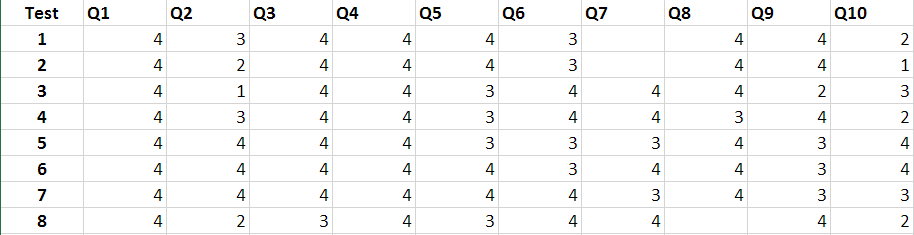
\includegraphics[width=1.00\textwidth]{media/tableData.png}
	\caption{Datenreihe des Fragebogens}
	\label{fig:tableData}
\end{figure}

\begin{figure}[h]
	\centering
		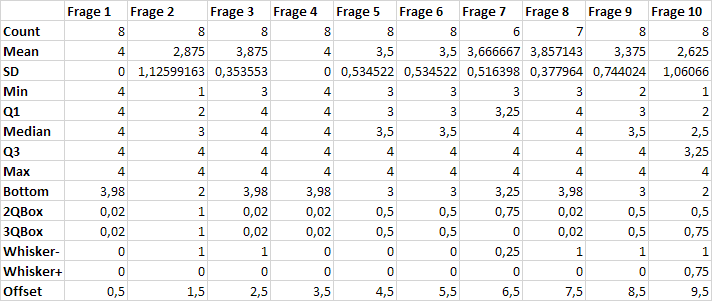
\includegraphics[width=1.00\textwidth]{media/excel_calculation.png}
	\caption{Berechnungen zur Auswertung des Fragebogens}
	\label{fig:excel_calculation}
\end{figure}


\clearpage

%*********************************************************************%
% Dokumente                                                           %
%*********************************************************************%
\refstepcounter{section}
\addcontentsline{toc}{section}{\protect\numberline{\thesection} Fragebogen}
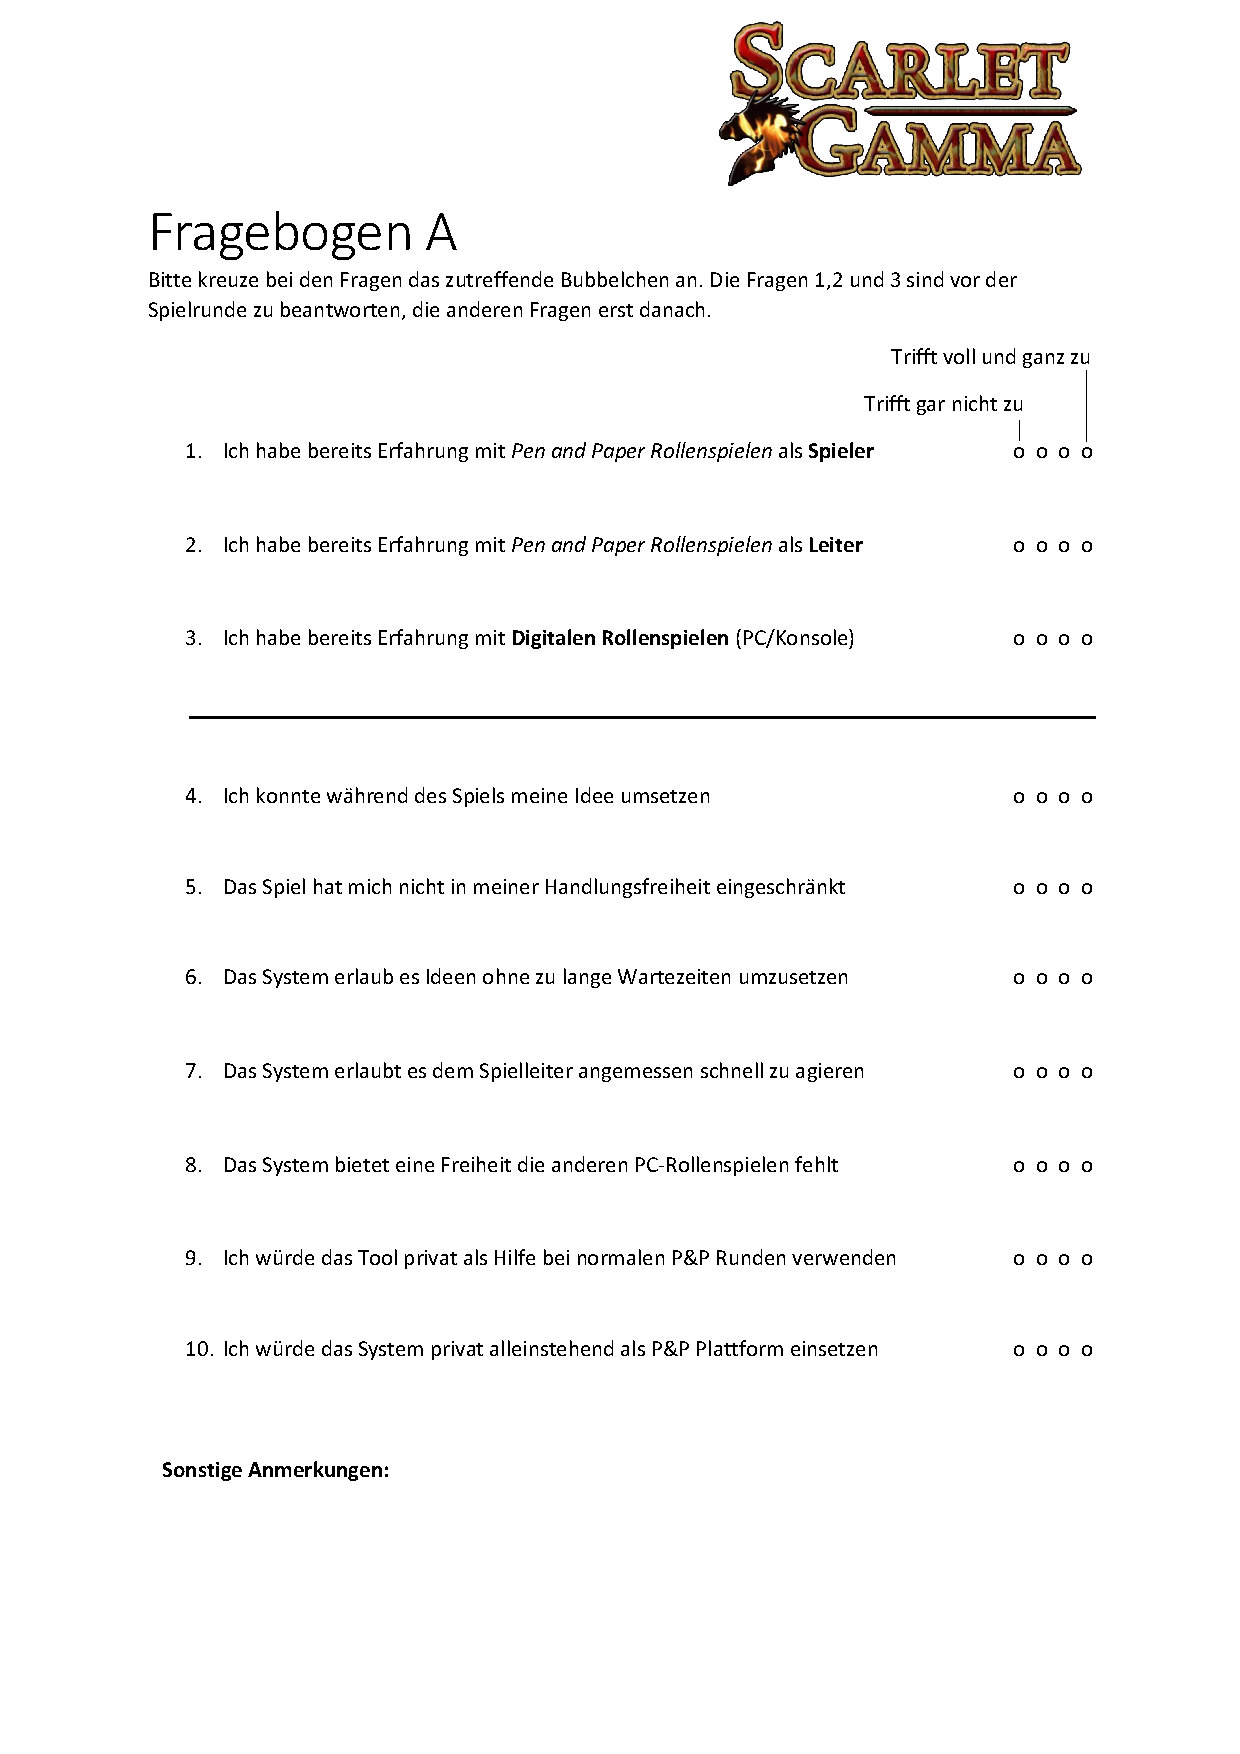
\includepdf[pages=-,link,linkname=AppendixFragebogenA]{../Fragebogen_A.pdf}
\refstepcounter{section}
\addcontentsline{toc}{section}{\protect\numberline{\thesection} Testszenario Spielleiter}
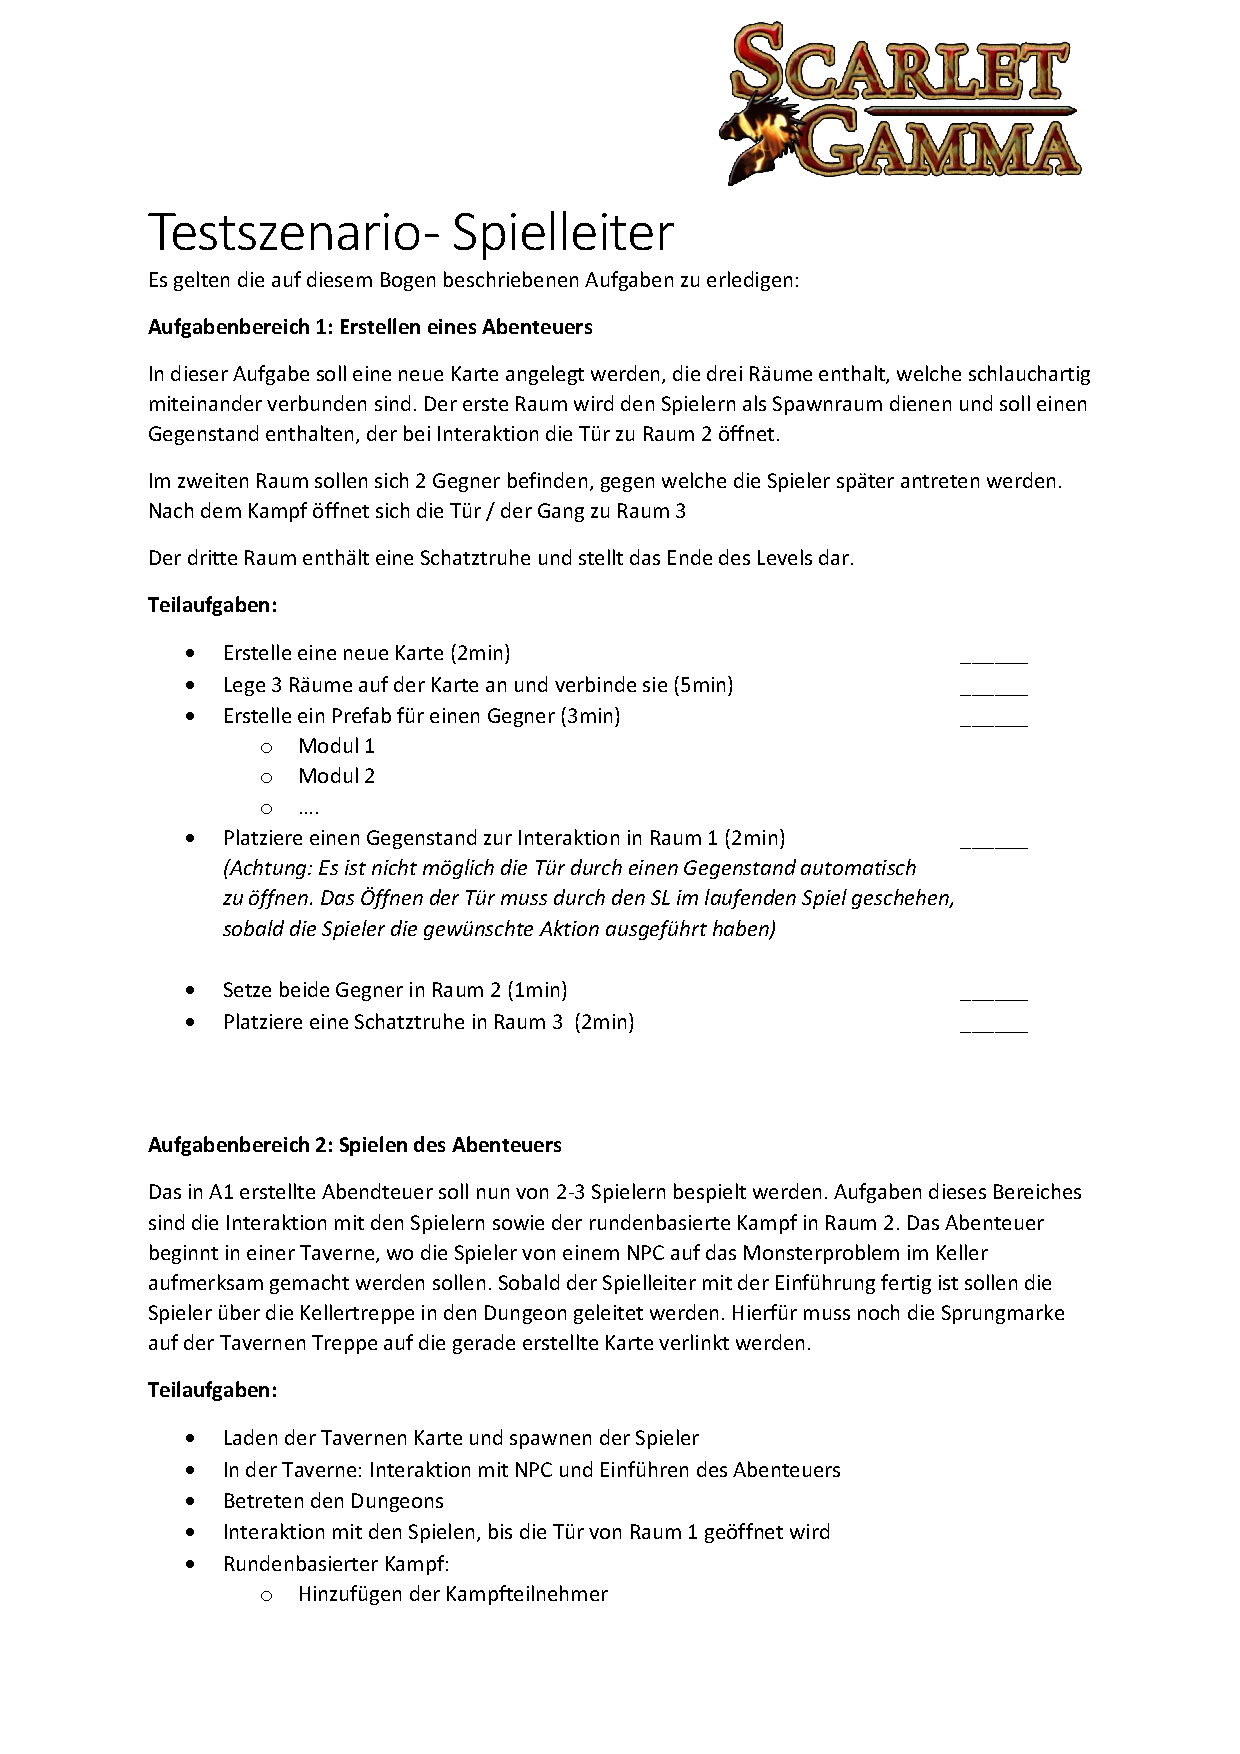
\includepdf[pages=-,link,linkname=AppendixSpielleiter]{../Testszenario_Spielleiter.pdf}
\refstepcounter{section}
\addcontentsline{toc}{section}{\protect\numberline{\thesection} Handbuch}
\includepdf[pages=-,link,linkname=AppendixManual]{../QuickManual/manual.pdf}


%*********************************************************************%
% LITERATURE                                                          %
%*********************************************************************%

\cleardoublepage
\phantomsection
\addcontentsline{toc}{chapter}{\bibname} % 
\bibliographystyle{geralpha} % plain gerplain abbrvnat unsrtnat alphag alpha
% in a thesis you have space... use full names
\bibliography{literature/literature}
% in a paper, space is limited. use abreviations
%\bibliography{../literature/IEEEabrv,../literature/MYabrv,../literature/literature}

%*********************************************************************%
% Dokumente                                                           %
%*********************************************************************%
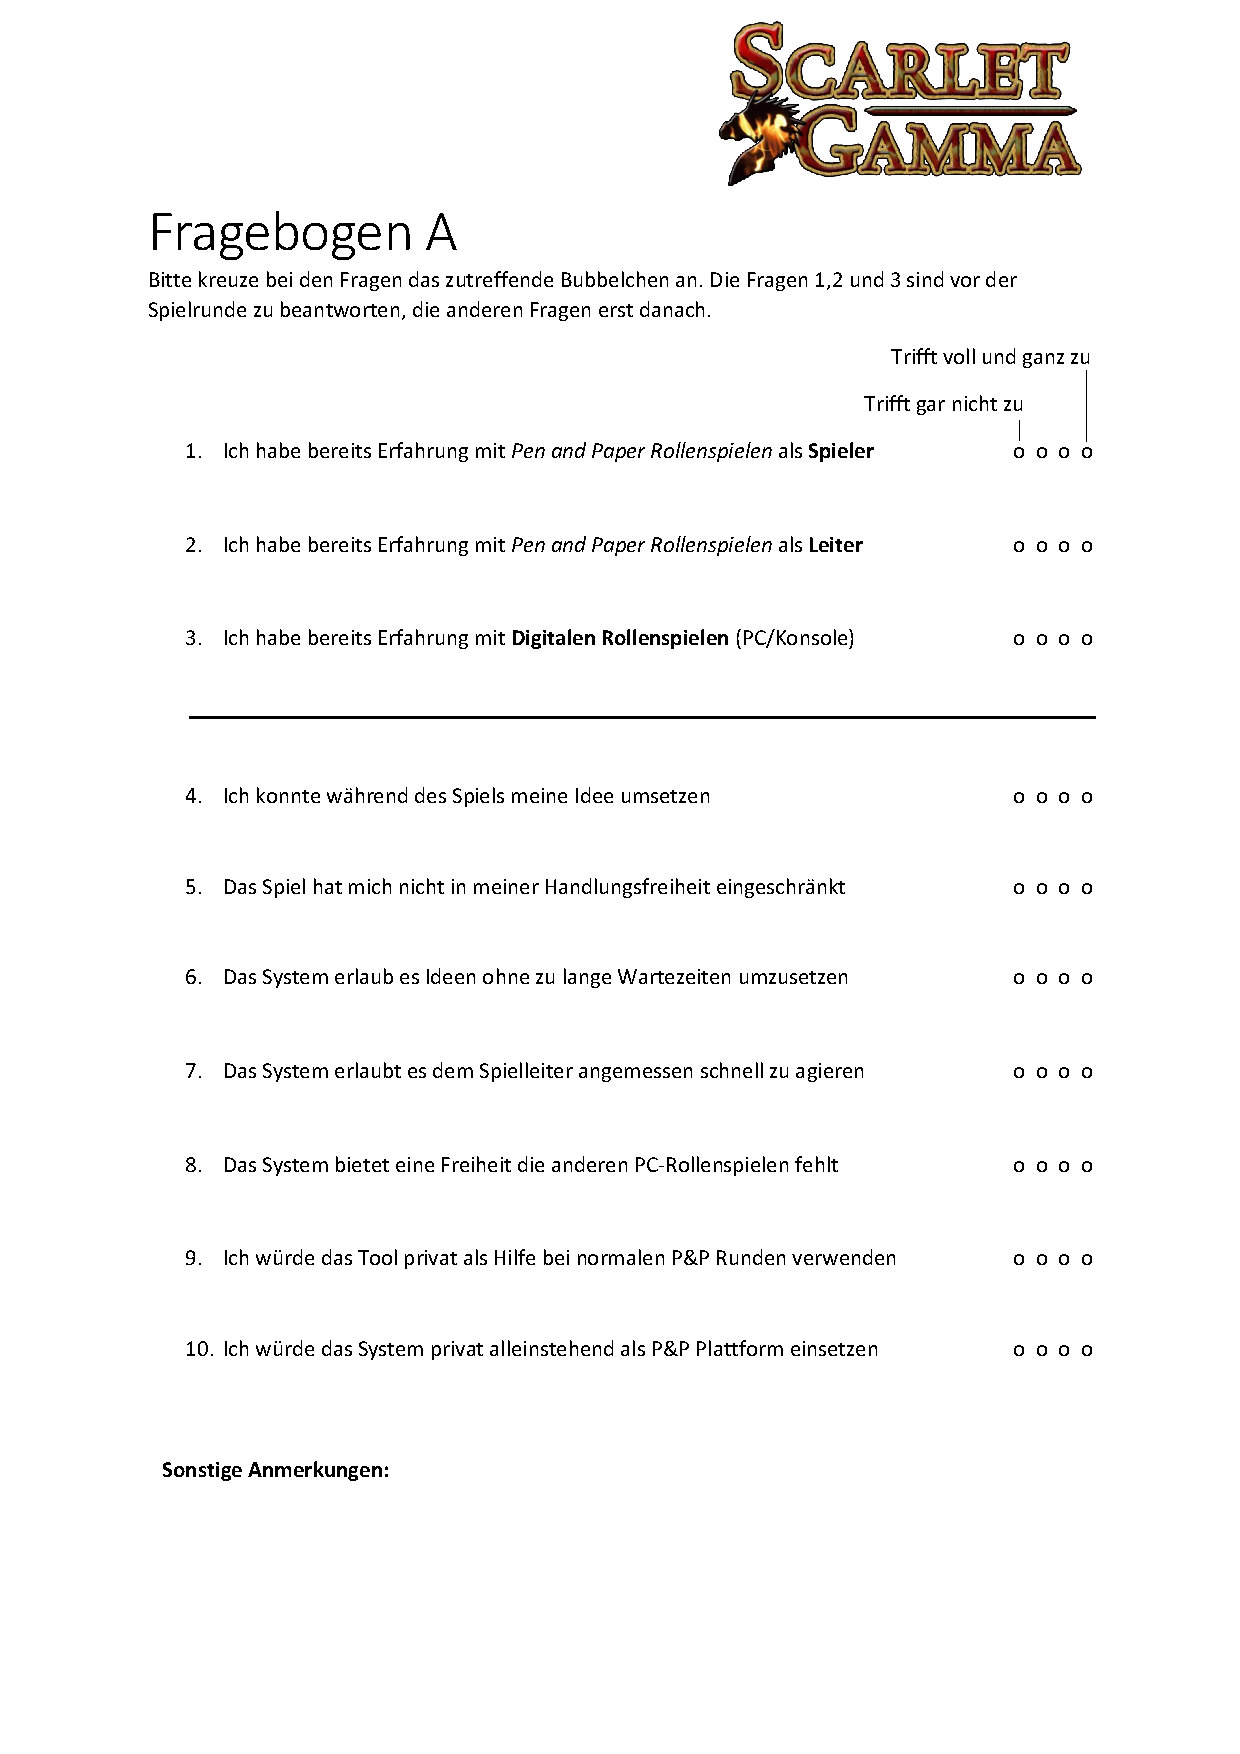
\includepdf[pages=-]{../Fragebogen_A.pdf}
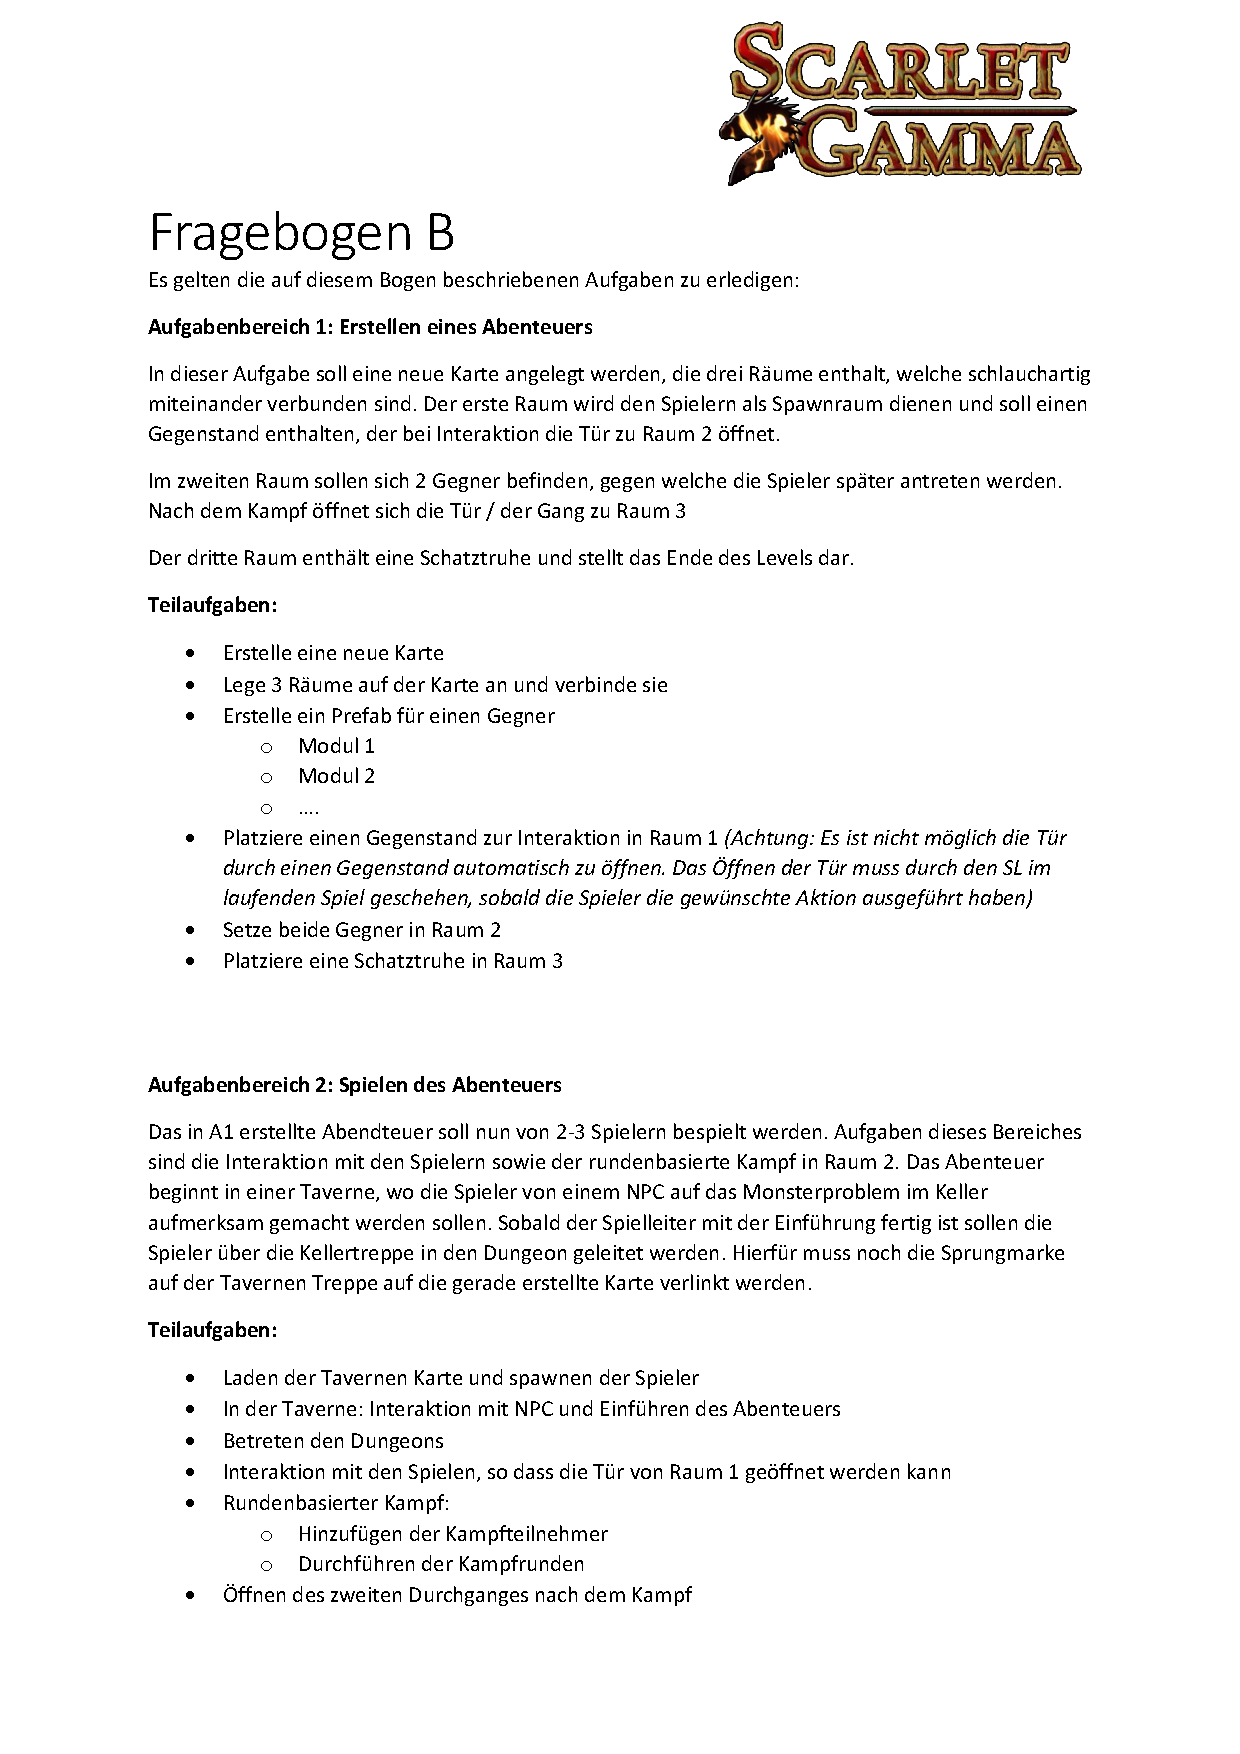
\includepdf[pages=-]{../Fragebogen_B.pdf}

%*********************************************************************%
% ERKLÄRUNG                                                           %
%*********************************************************************%

\ifnotdraft {
	\cleardoublepage
	\phantomsection
}
\printindex

\ifnotdraft{
	\thispagestyle{empty}
\vspace*{38\baselineskip}
\hbox to \textwidth{\hrulefill}
\par
Hiermit erkl\"are ich, dass ich die vorliegende Arbeit selbst\"andig verfasst und
keine anderen als die angegebenen Quellen und Hilfsmittel verwendet habe.

Magdeburg, den 21.3.2014

%%%%%%%%%%%%%%%%%%%%%%%%%%%%%%%%%%%%%%%%%%%%%%%%%%%%%%%%%%%%%%%%%%%%%%%%
%% Hinweis:
%%
%% Diese Erklärung wird von der Prüfungsordnung für Diplomarbeiten 
%% verlangt und ist zu unterschreiben. Für Studienarbeiten ist diese
%% Erklärung nicht zwingend notwendig, schadet aber auch nicht.
%%%%%%%%%%%%%%%%%%%%%%%%%%%%%%%%%%%%%%%%%%%%%%%%%%%%%%%%%%%%%%%%%%%%%%%%
\clearpage

}

\end{document}
